\documentclass{beamer}
\pdfoutput=1

% The actual contents of the presentation begin much later.
% Look for the banner "TITLE SLIDE" below.

%----------
% PACKAGES
%----------

\usepackage{amssymb, amsmath, amsthm, graphicx}
\usepackage{mathtools}
\usepackage{color}
% Change the default serif font to one with heavier lines
\usepackage{mathptmx}

%----------------
% BEAMER OPTIONS
%----------------

% Remove navigation symbols; no one uses them, ever!
\setbeamertemplate{navigation symbols}{}

% General convention: MCL posters and presentations use serif fonts
\usefonttheme{serif}


%----------------
% THEOREM STYLES
%----------------

\theoremstyle{theorem}
\newtheorem{cor}{Corollary}
\newtheorem{prop}{Proposition}
\newtheorem{thm}{Theorem}
\newtheorem{lem}{Lemma}

\theoremstyle{definition}
\newtheorem*{remark}{Remark}
\newtheorem*{notation}{Notation}

% Others already defined in amsthm:
%   definition
%   example

%---------------------------
% COMMON SYMBOLS AND MACROS
%---------------------------

\newcommand{\R}{\mathbb{R}}
\newcommand{\Z}{\mathbb{Z}}
\newcommand{\N}{\mathbb{N}}
\newcommand{\C}{\mathbb{C}}

% Real and imaginary part
\DeclareMathOperator{\im}{Im}
\DeclareMathOperator{\re}{Re}

\newcommand{\into}{\hookrightarrow}
\newcommand{\tensor}{\otimes}

\newcommand{\req}{\renewcommand{\theequation}{\thechapter.\arabic{equation}}}
\newcommand{\sol}{\hspace{-0.7cm}\textbf{\textit{Solu��o:}}}
\newcommand{\barr}[1]{\overline{#1}}
\newcommand{\tq}{\mid}
\newcommand{\ifff}{if, and only if }
\newcommand{\xsi}{1+\xi\bar{\xi}}
\newcommand{\dxsi}{\dfrac{\partial}{\partial\xi}}
\newcommand{\dxsib}{\dfrac{\partial}{\partial\overline{\xi}}}
\newcommand{\jacob}{\partial^- F\overline{\partial^- F}-\partial^+ F\overline{\partial^+ F}}
\newcommand{\jaco}{\partial^- F\overline{\partial^- F}+\partial^+ F\overline{\partial^+ F}}
\newcommand{\p}{\partial}
\newcommand{\cqd}{ \begin{flushright} $\square$ \end{flushright}}

%-----------------
% ASSORTED TWEAKS
%-----------------

% Use less/greater than or equal to with slanted, not horizontal line
% by default
\renewcommand{\leq}{\leqslant}
\renewcommand{\geq}{\geqslant}


%======================================================================
%                          TITLE SLIDE
%======================================================================

\title{
	Wikipedia Illustration Task Force \\
	\large Visualizing Kempe's Universality Theorem}
\author{Student Researchers: Amy Herz, Jacob Krol \\
	Faculty Supervisor: Jan Verschelde}
%\author{Anne K. Example\\Second J. Author}
\institute{}
\date{October 25, 2017}
%\date{\today}

\titlegraphic{
\vspace{0.1\paperheight}
\hspace{0.03\paperwidth}

\includegraphics[keepaspectratio=true,height=0.15\paperheight]{logo-wordmark}
\hfill

\includegraphics[keepaspectratio=true,height=0.15\paperheight]{uiclogo.pdf}
\hspace{0.03\paperwidth}
}

\begin{document}
\frame{\titlepage}


%======================================================================
%                          CONTENT SLIDES
%======================================================================

\begin{frame} % frame = slide in beamer terminology
\frametitle{Kempe's Universality Theorem}
\begin{thm}
For an arbitrary algebraic plane curve a linkage can be constructed that draws the curve.
\end{thm}

\begin{center}
\begin{figure}
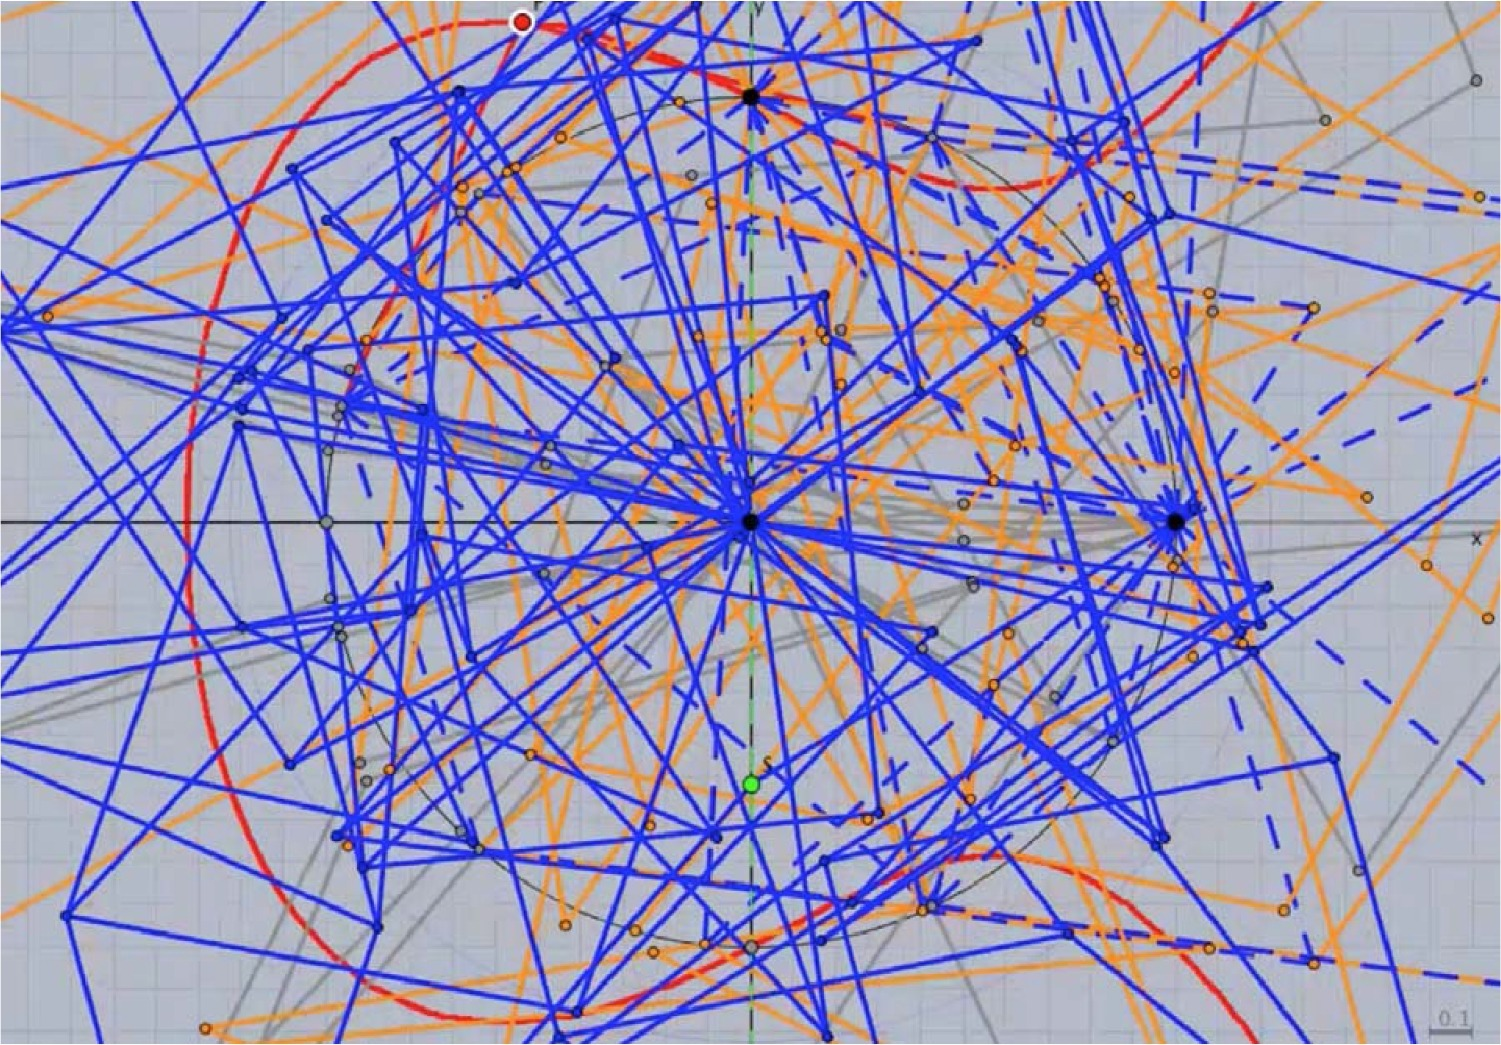
\includegraphics[keepaspectratio=true,height=0.5\paperheight]{quad-curve}
\end{figure}
\end{center}

\end{frame}

%=====================================================================

\begin{frame}
\frametitle{Trigonometric Plane Curves}

\begin{definition}
A trigonometric plane curve, $P=(x(\theta),y(\theta))$, is a parameterized curve with coordinate functions that are finite Fourier series. 
\end{definition}

\begin{example}
\[
P_{T}=\begin{rcases}
	\begin{dcases} 
	-\cos{2\theta} - \cos{4\theta}\\
	\sin{2\theta} - \sin{4\theta}
	\end{dcases}
	\end{rcases}
\]
\end{example}

\end{frame}

%=====================================================================

\begin{frame}
\frametitle{Mechanisms to Draw Trigonometric Plane Curves}

\begin{definition}
A single-coupled serial chain is a mechanism that can be realized by coupling successive joint rotations of a serial chain linkage, using gears or cable-pulley drives. 
\end{definition}

%\vspace{1mm}

\begin{itemize}
\item all links in a single-coupled serial chain are connected to the same input angle $\theta$
\item cable drives at increasing speeds by pulleys of decreasing radius
\end{itemize}

\begin{columns}

\begin {column} {0.5\textwidth}
	\begin{center}
		\begin{figure}
		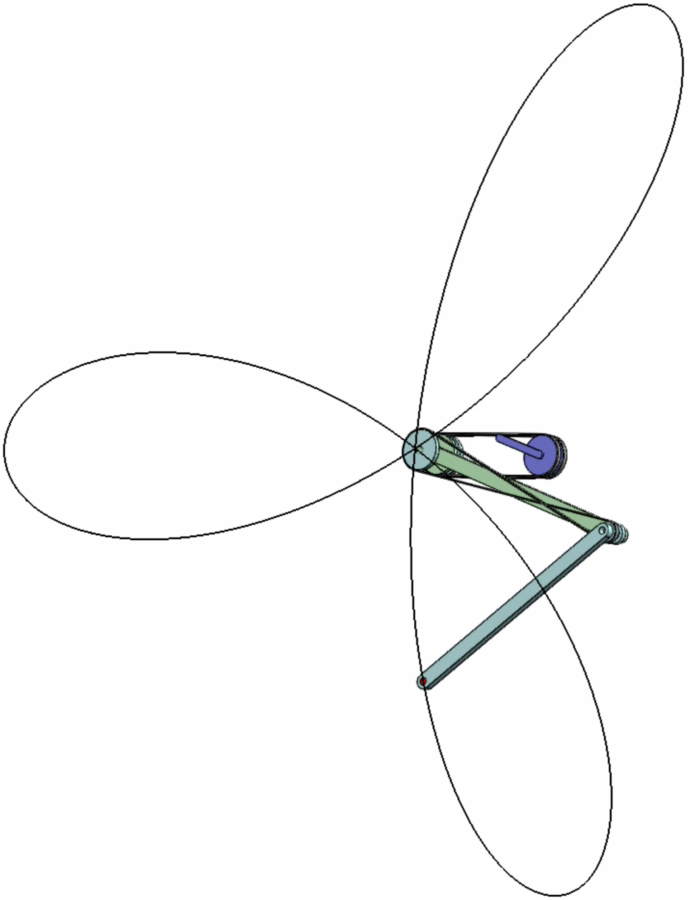
\includegraphics[keepaspectratio=true,height=0.3\paperheight]{trifolium-serialchain}
		\end{figure}
	\end{center}
\end{column}

\begin{column} {0.5\textwidth}
	\begin{center}	
	\begin{figure}
	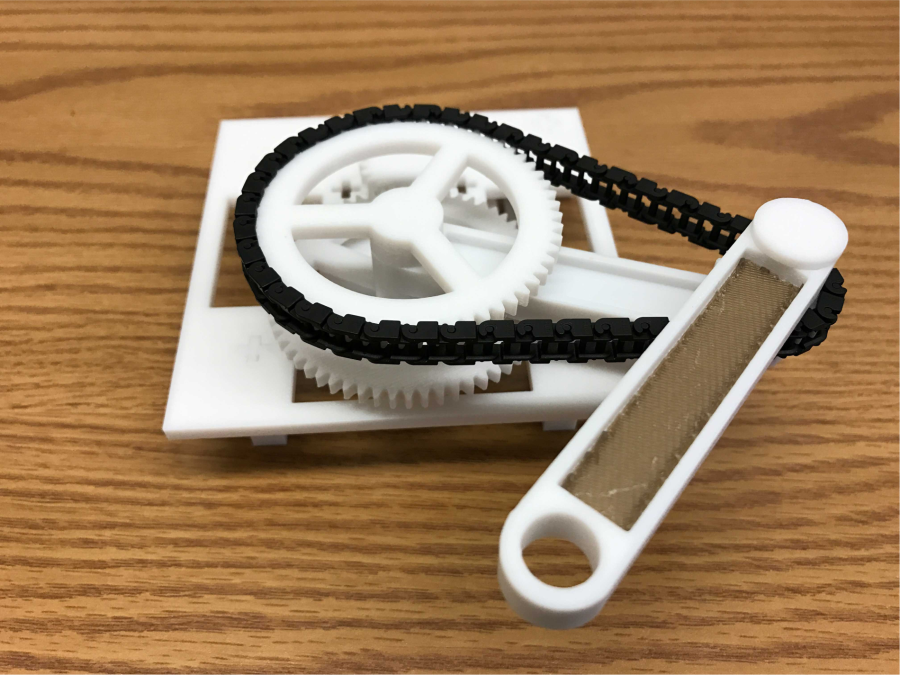
\includegraphics[keepaspectratio=true,height=0.3\paperheight]{tri-mechanism}
	\end{figure}
	\end{center}
\end{column}
\end{columns}

\end{frame}
%======================================================================
%                          ANIMATION SLIDES
%======================================================================

\begin{frame}
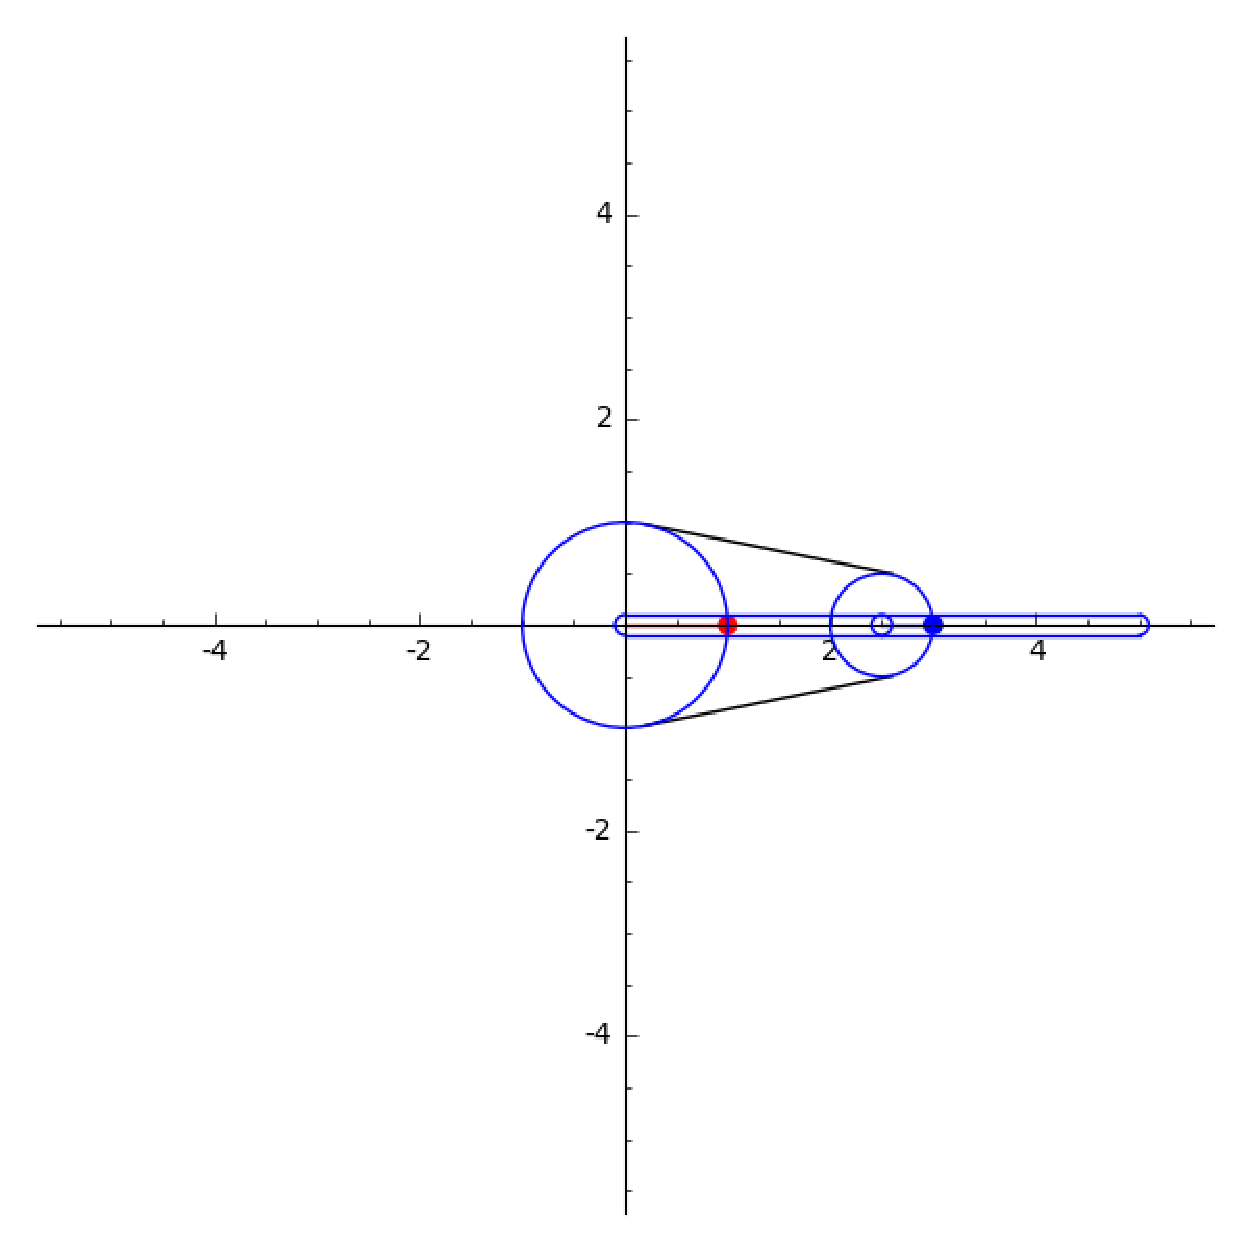
\includegraphics[scale=0.5]{tri1.eps}
\end{frame}

\begin{frame}
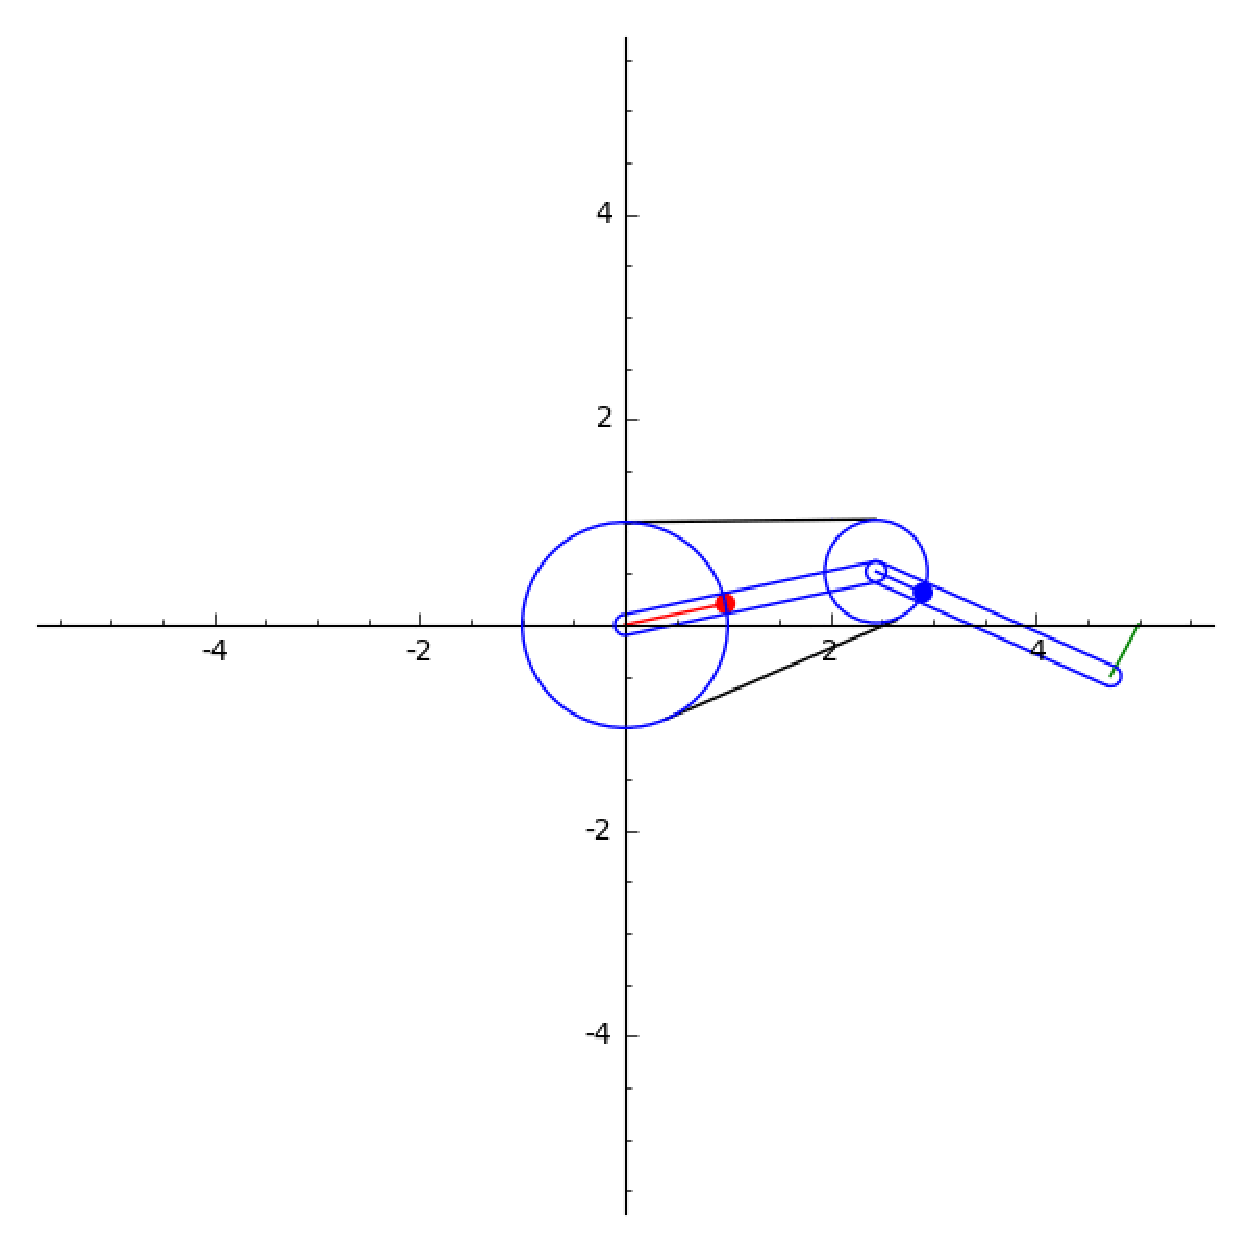
\includegraphics[scale=0.5]{tri2.eps}
\end{frame}

\begin{frame}
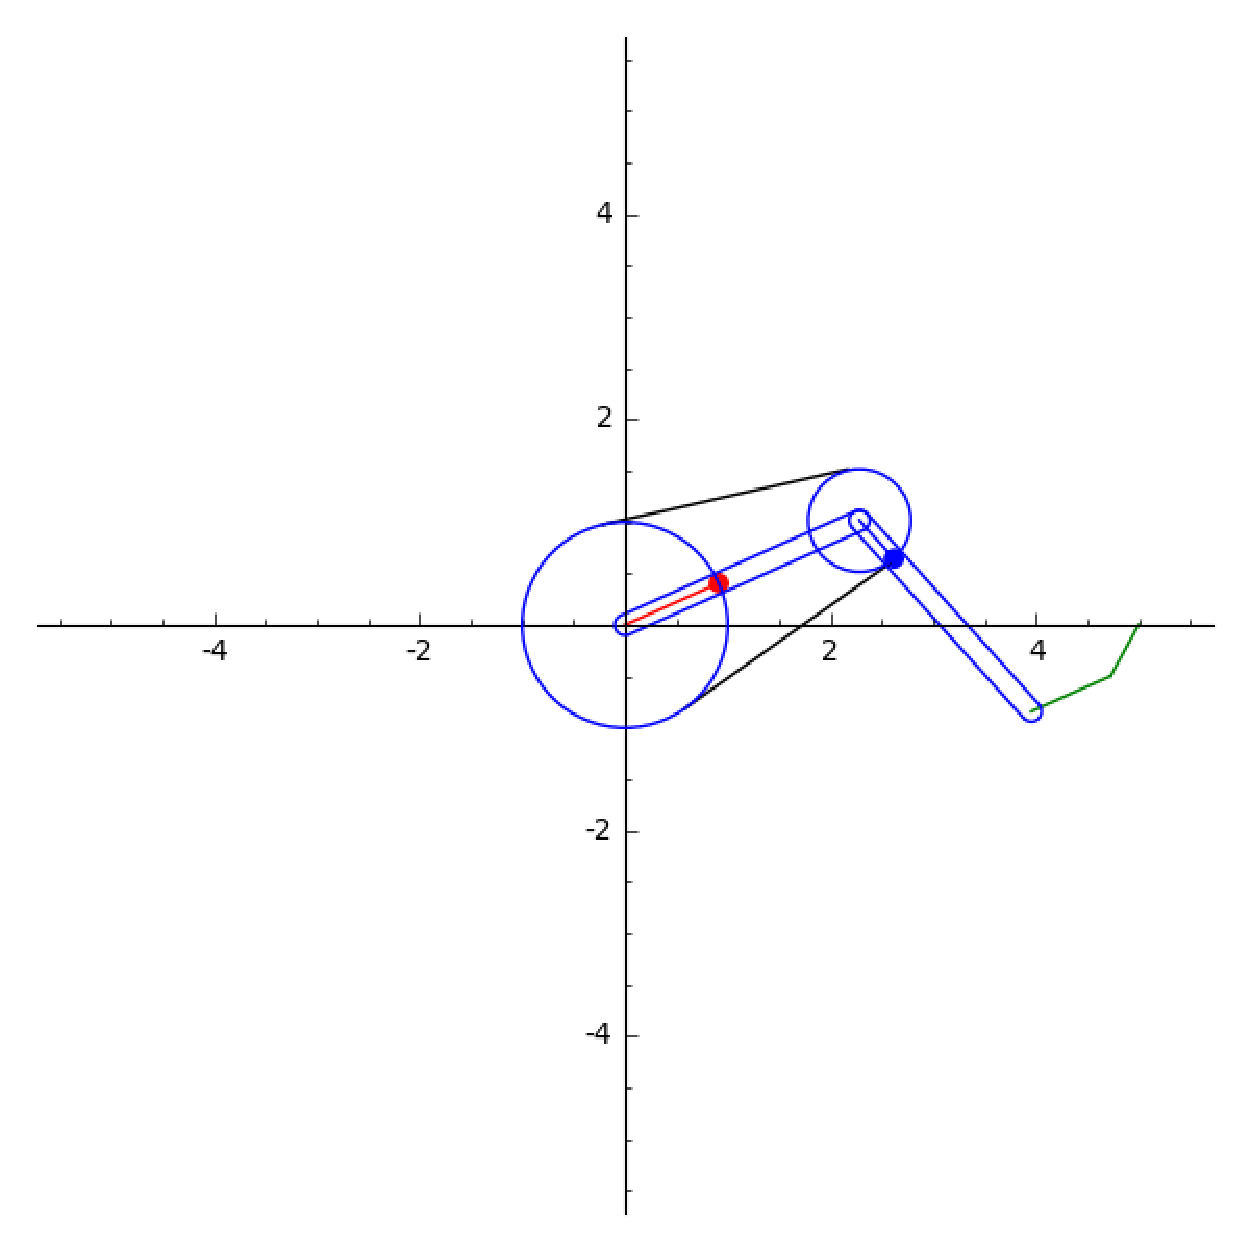
\includegraphics[scale=0.5]{tri3.eps}
\end{frame}

\begin{frame}
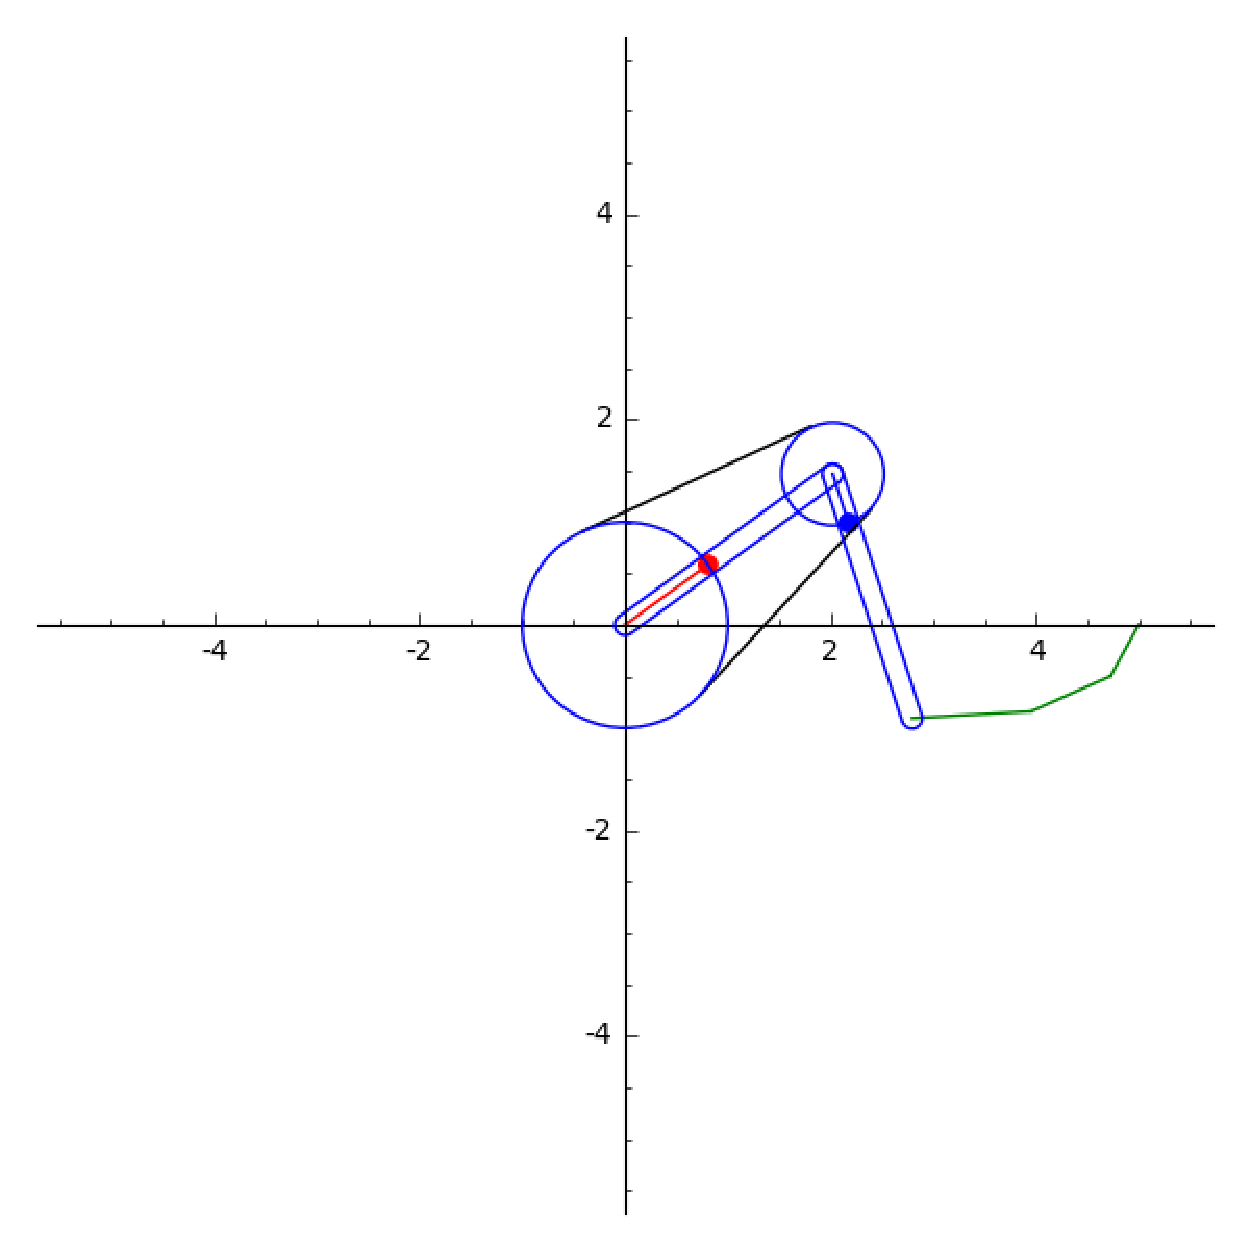
\includegraphics[scale=0.5]{tri4.eps}
\end{frame}

\begin{frame}
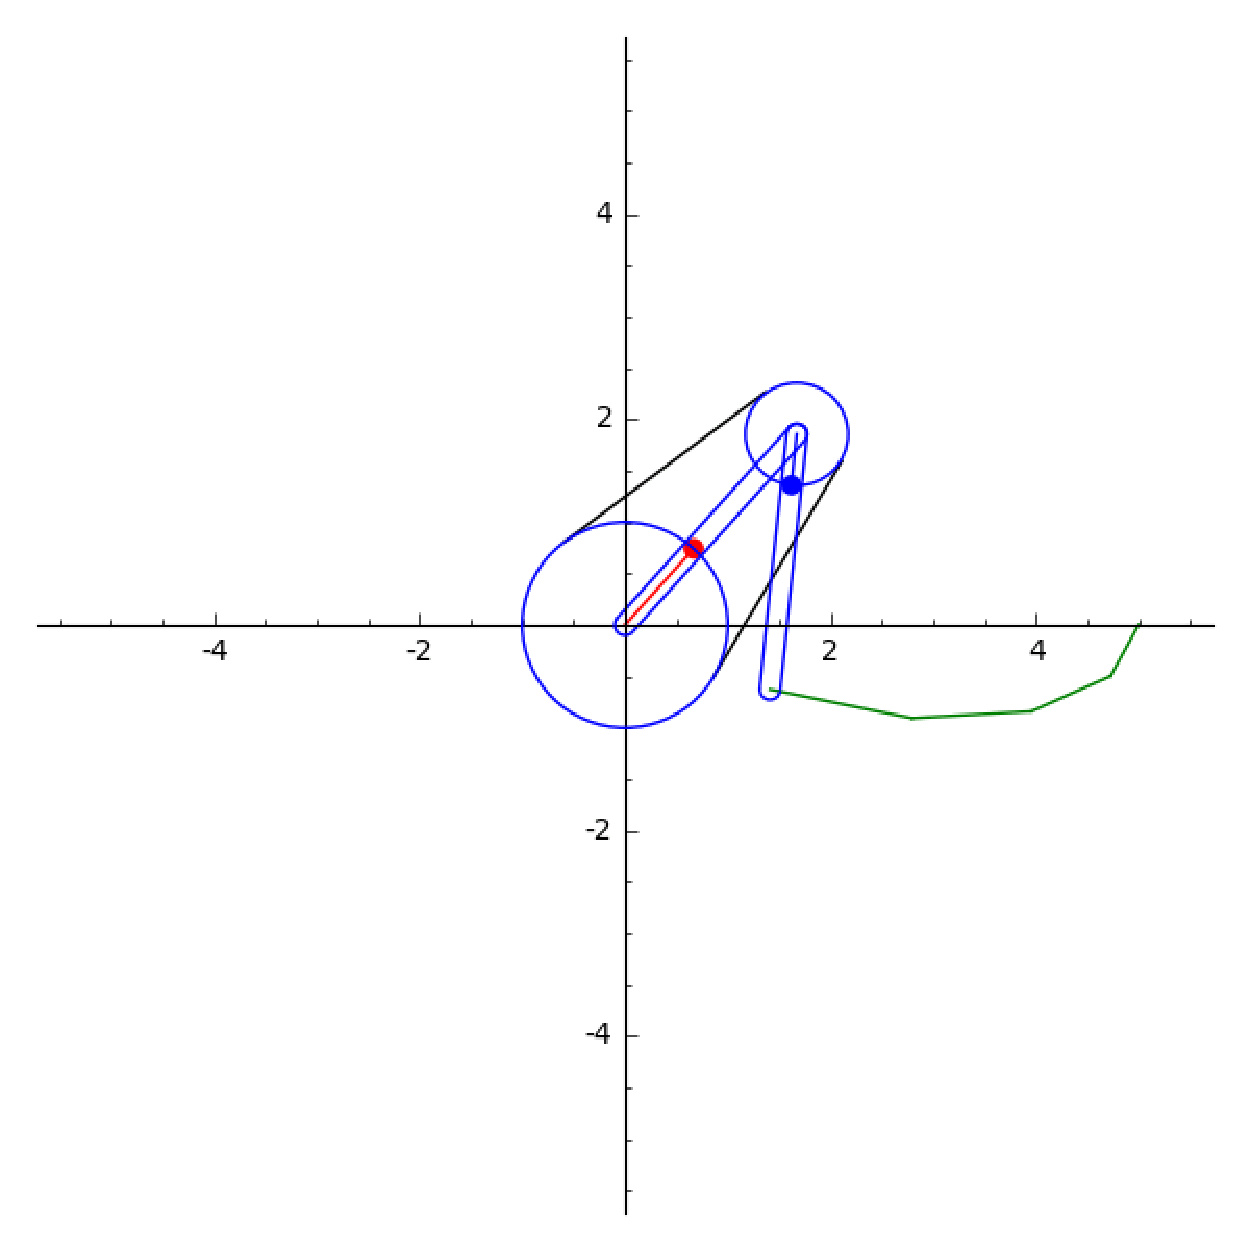
\includegraphics[scale=0.5]{tri5.eps}
\end{frame}

\begin{frame}
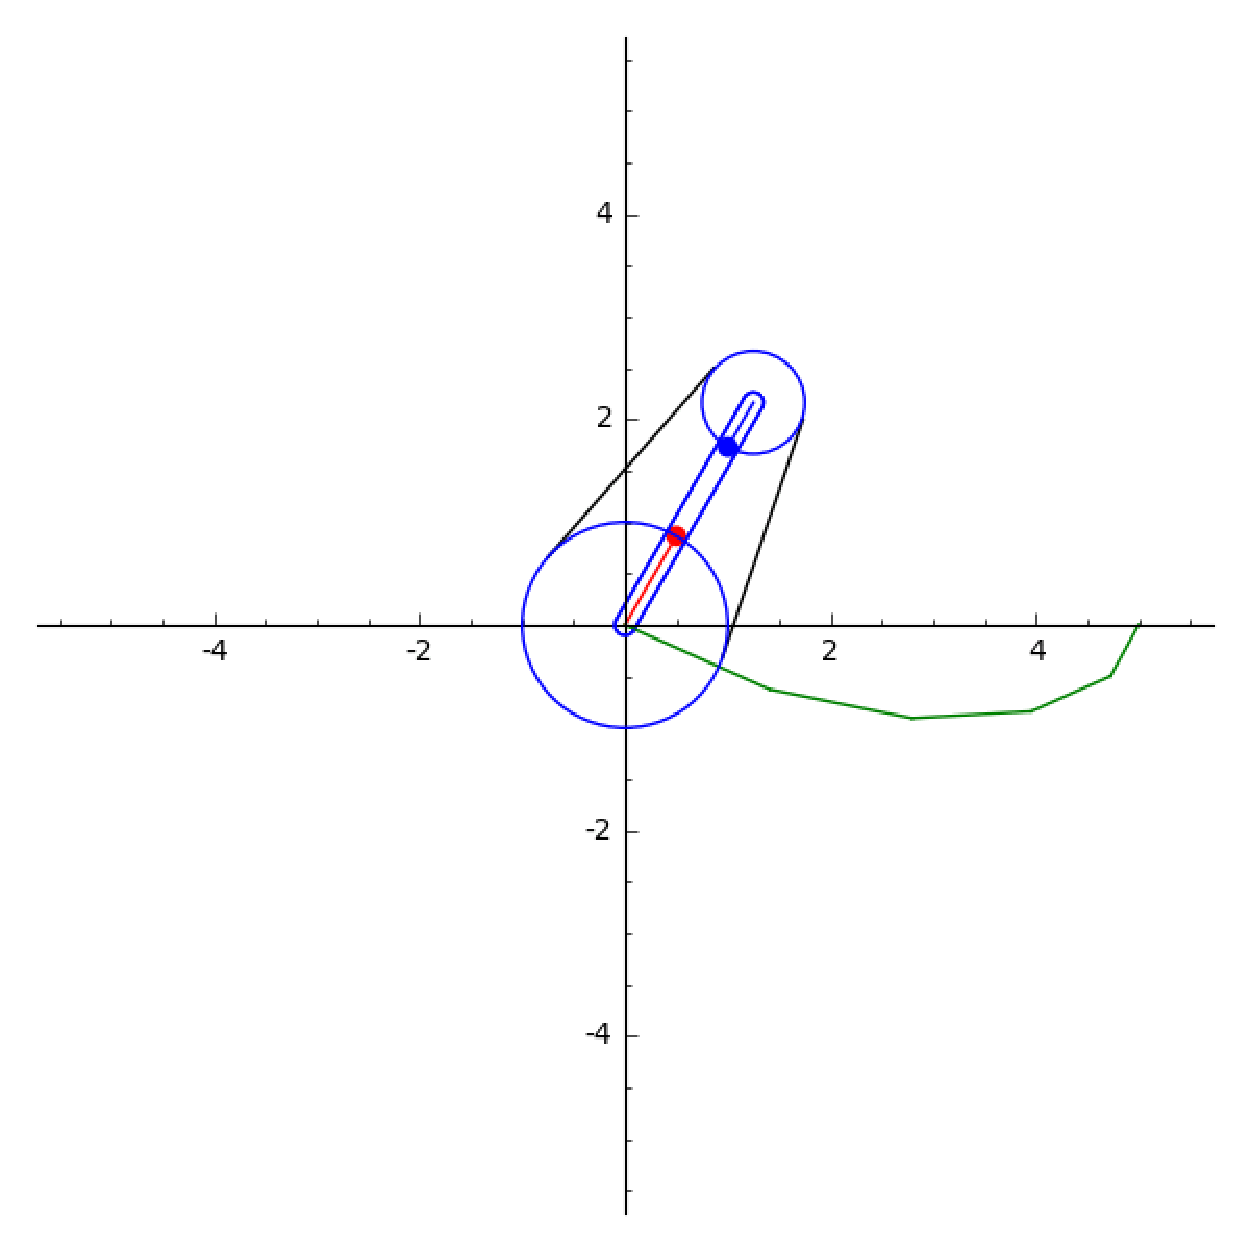
\includegraphics[scale=0.5]{tri6.eps}
\end{frame}

\begin{frame}
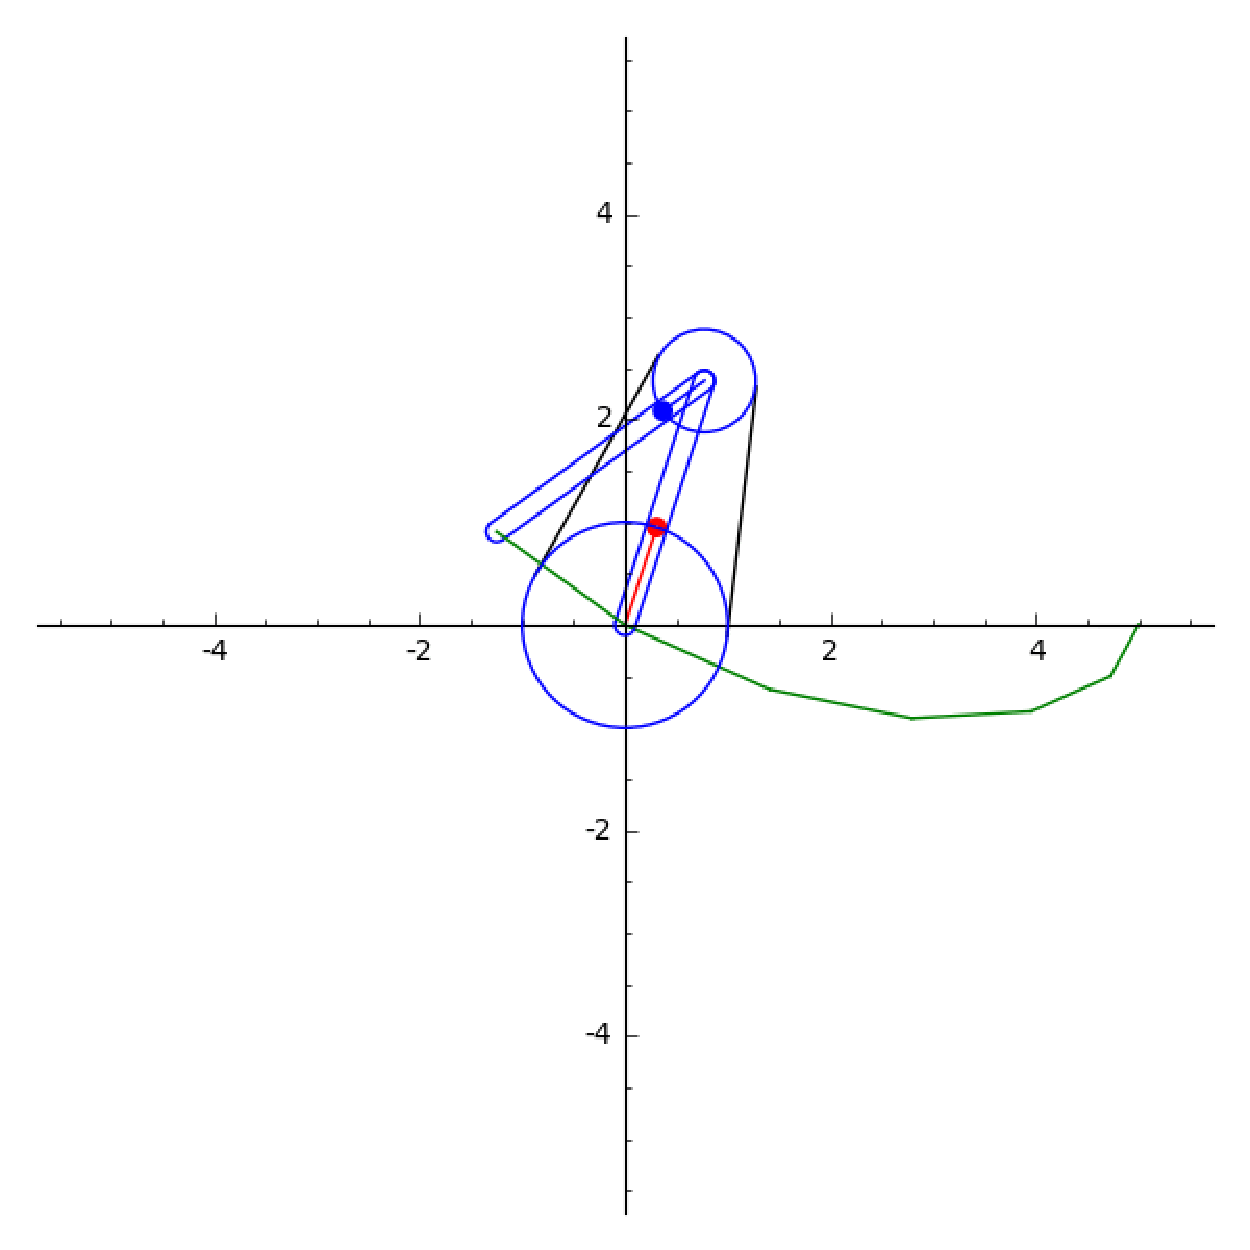
\includegraphics[scale=0.5]{tri7.eps}
\end{frame}

\begin{frame}
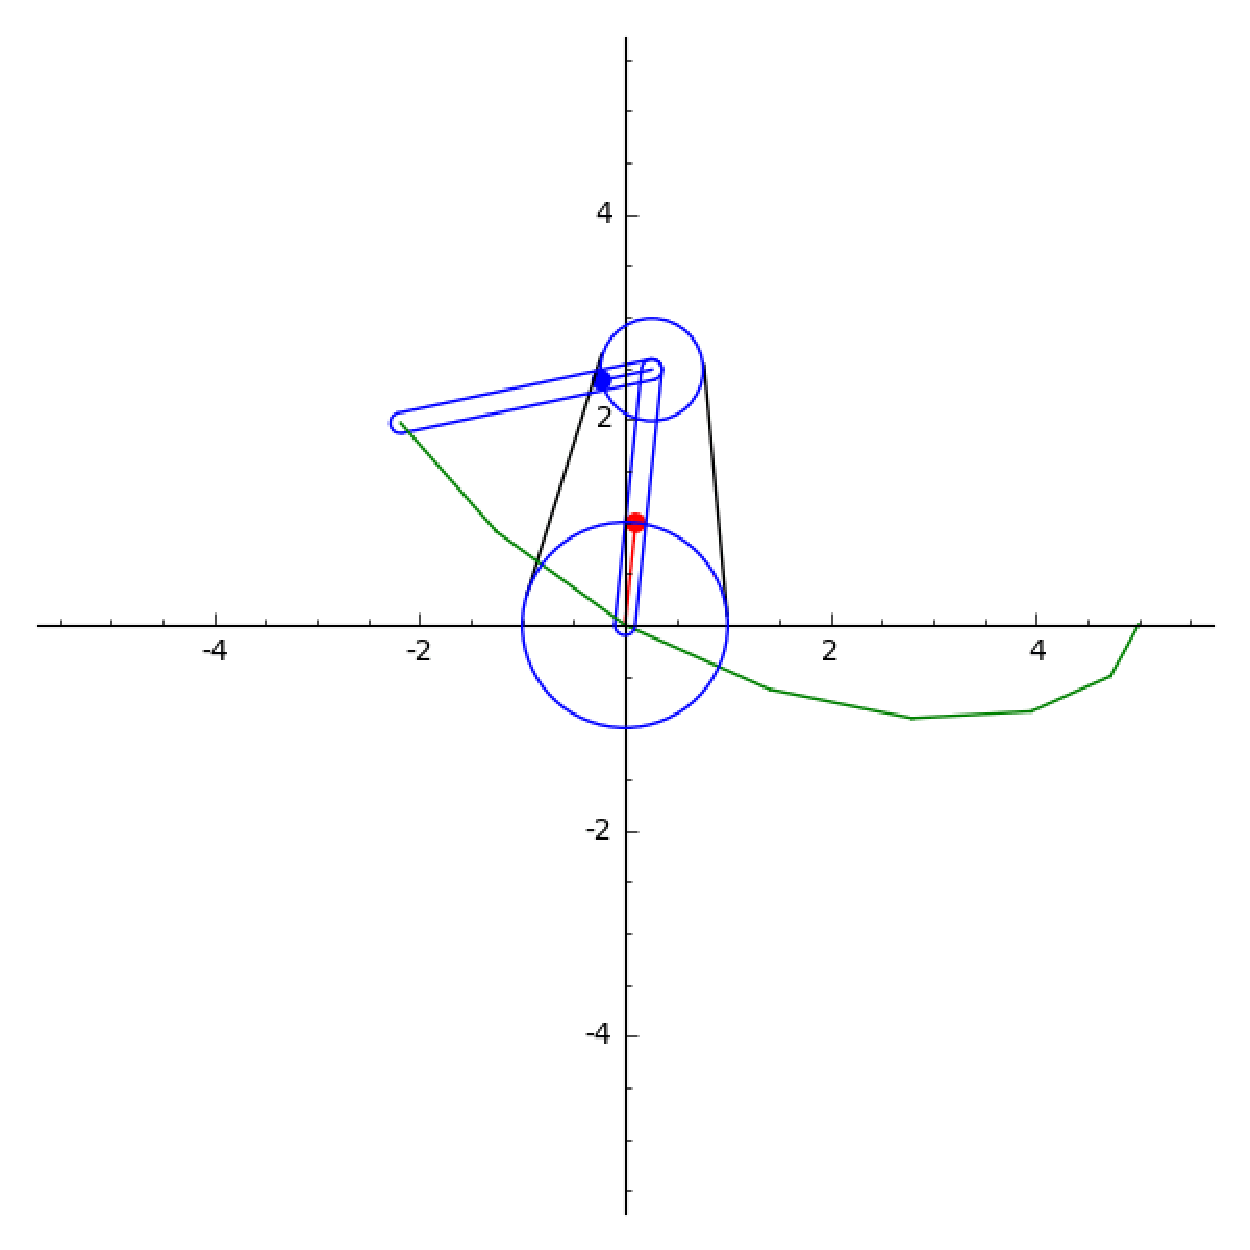
\includegraphics[scale=0.5]{tri8.eps}
\end{frame}

\begin{frame}
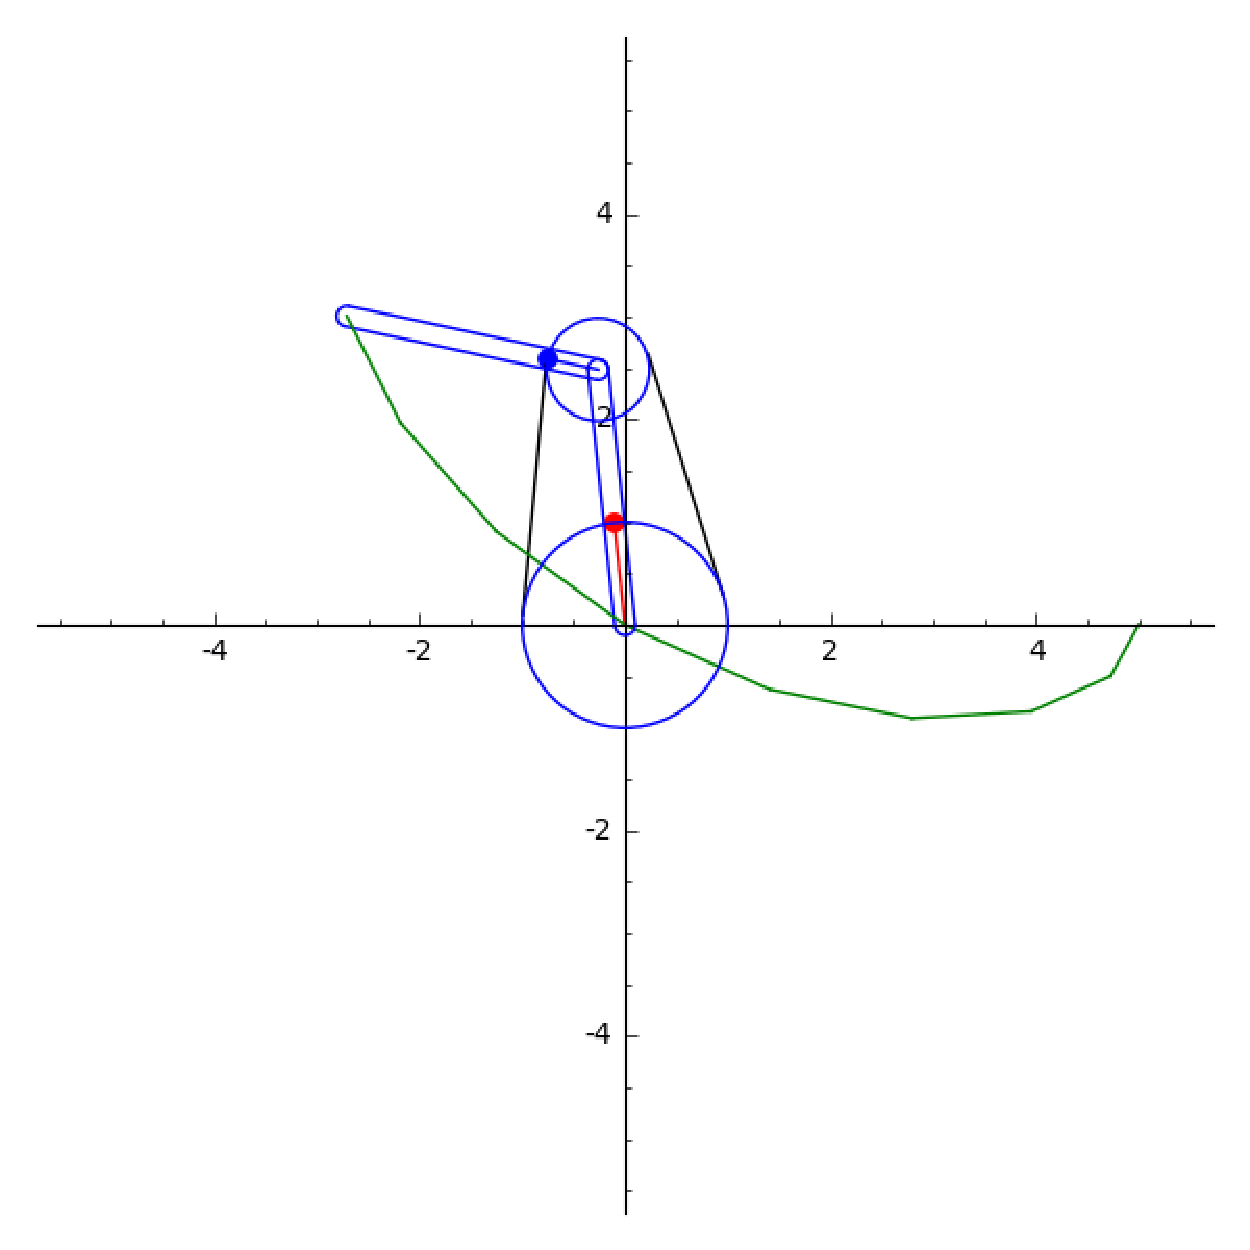
\includegraphics[scale=0.5]{tri9.eps}
\end{frame}

\begin{frame}
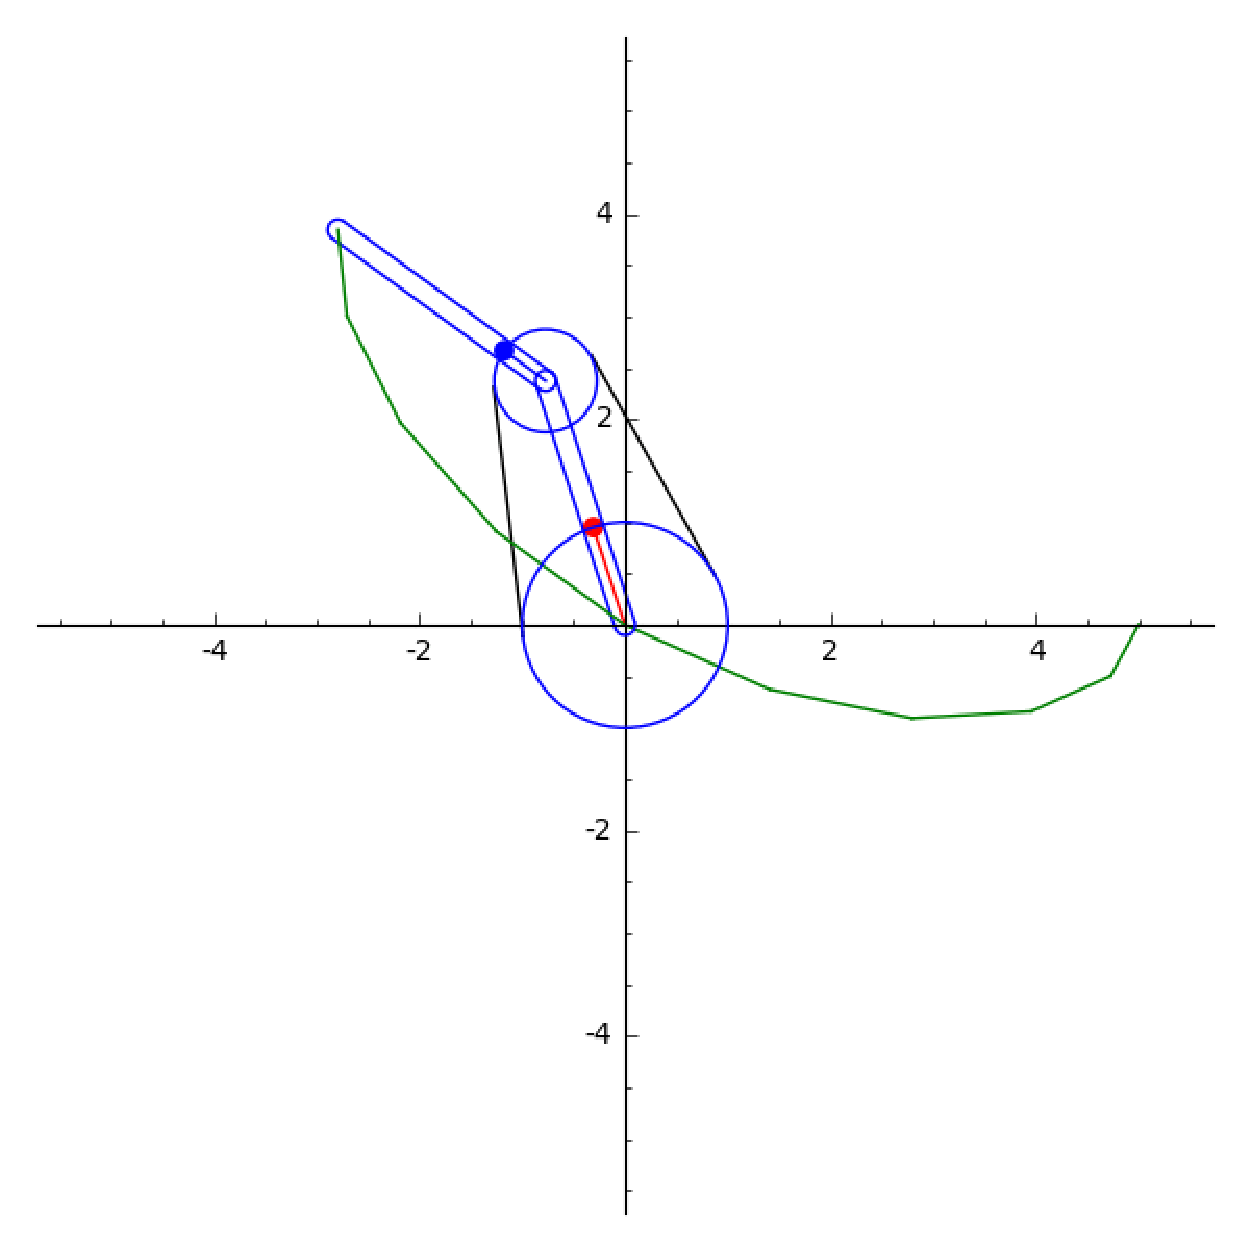
\includegraphics[scale=0.5]{tri10.eps}
\end{frame}

\begin{frame}
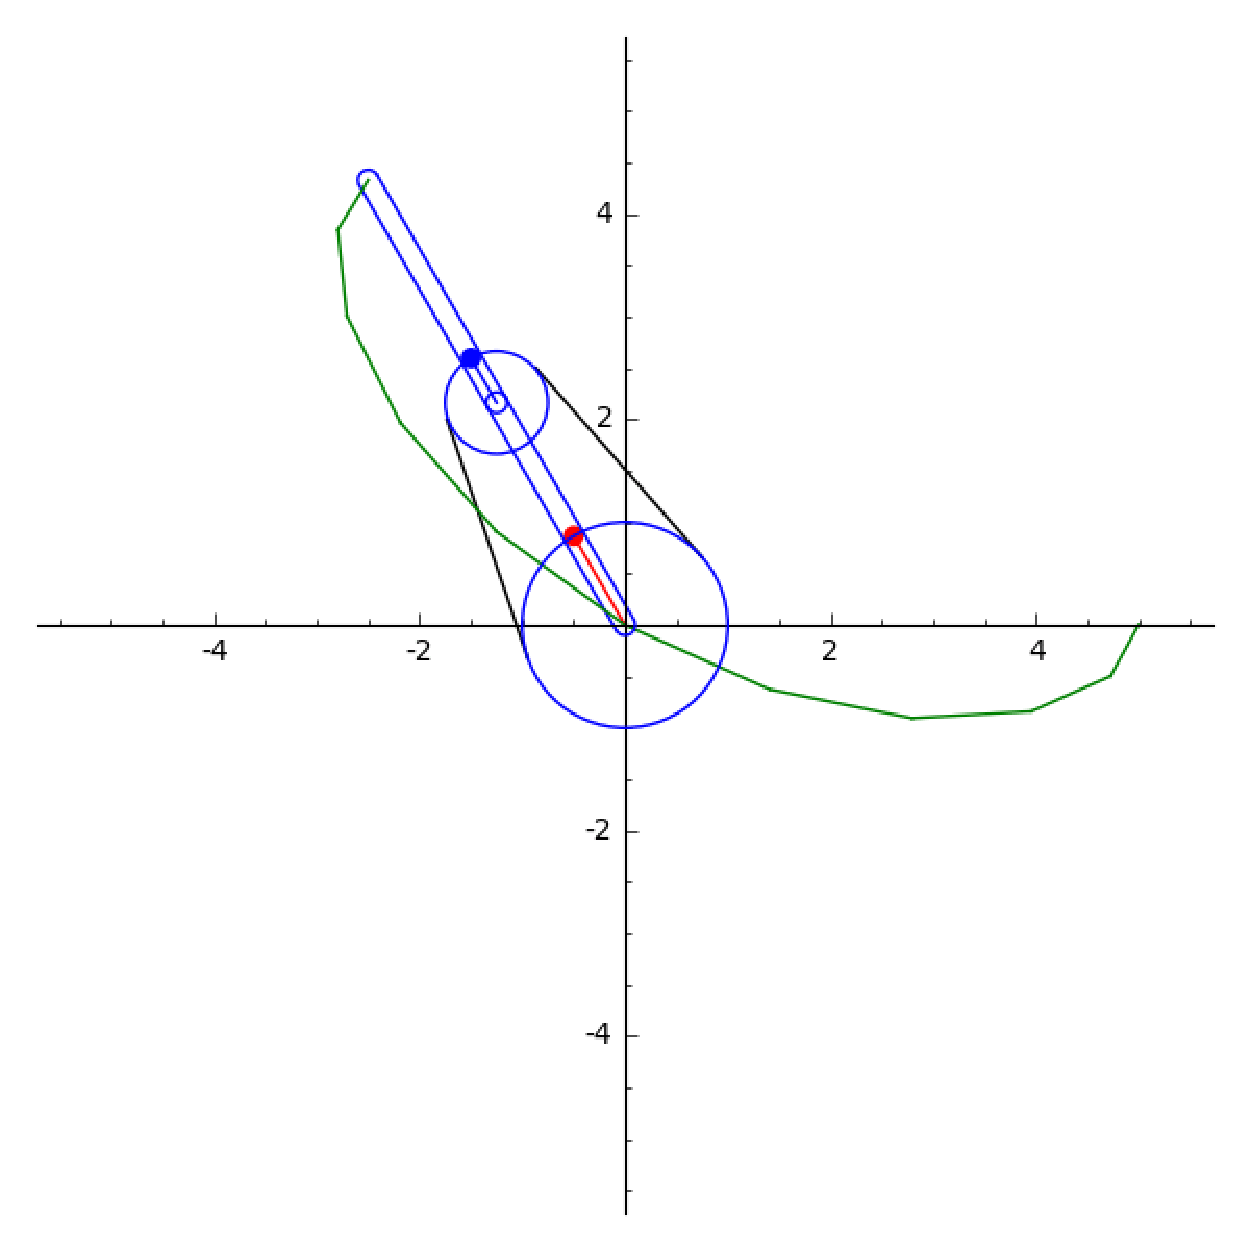
\includegraphics[scale=0.5]{tri11.eps}
\end{frame}

\begin{frame}
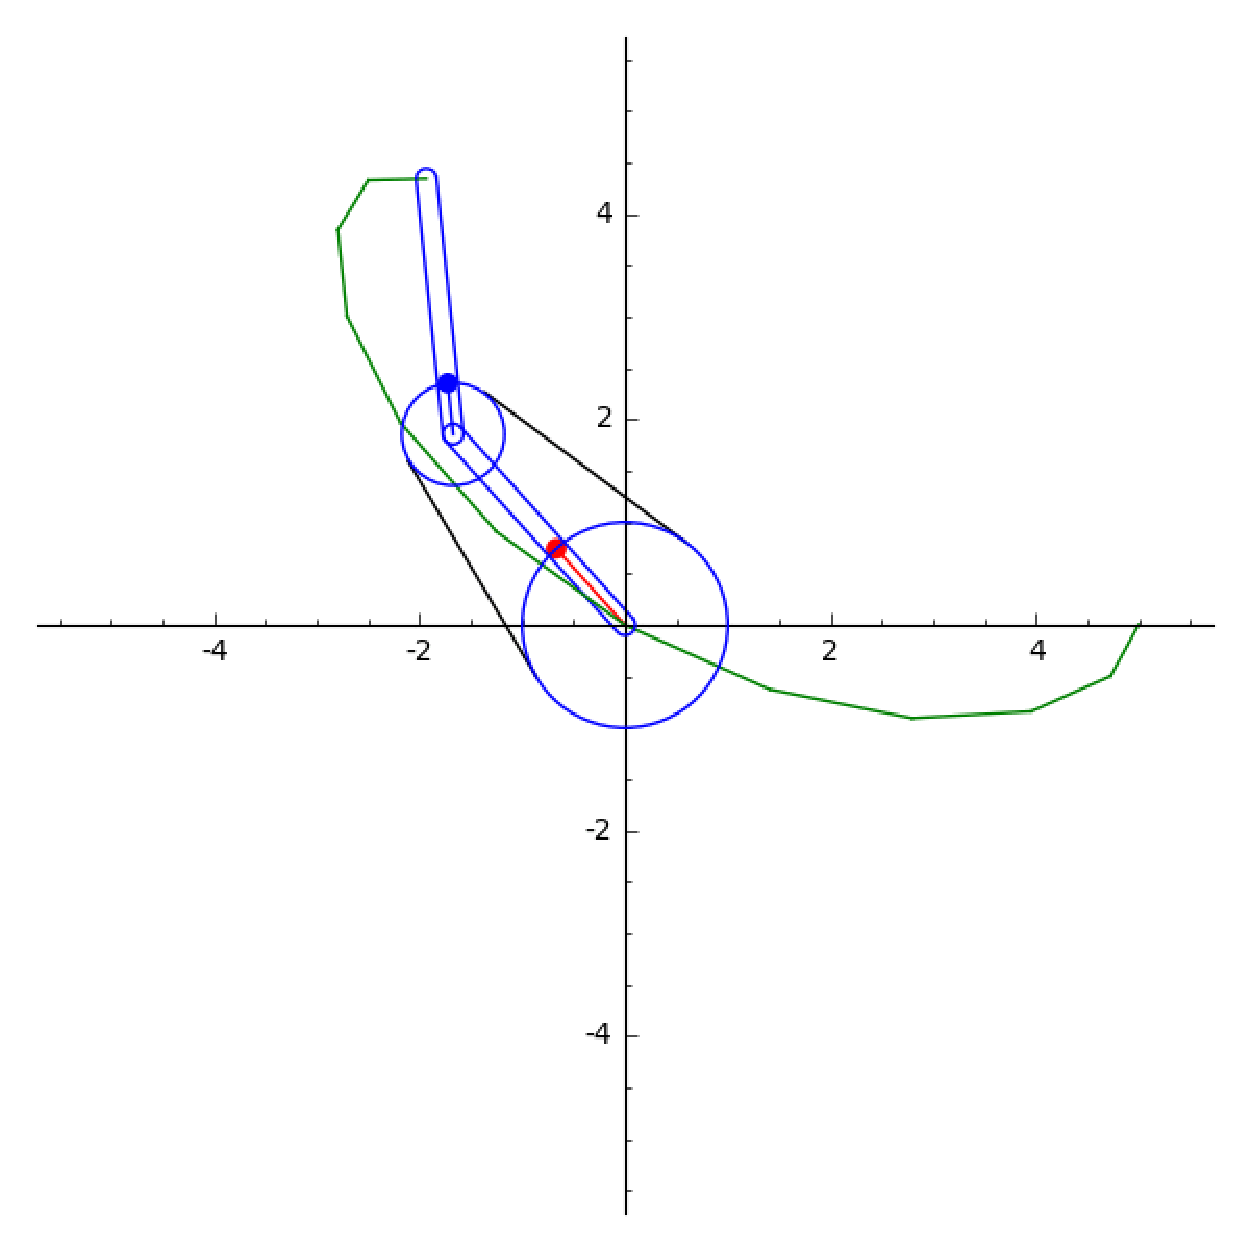
\includegraphics[scale=0.5]{tri12.eps}
\end{frame}

\begin{frame}
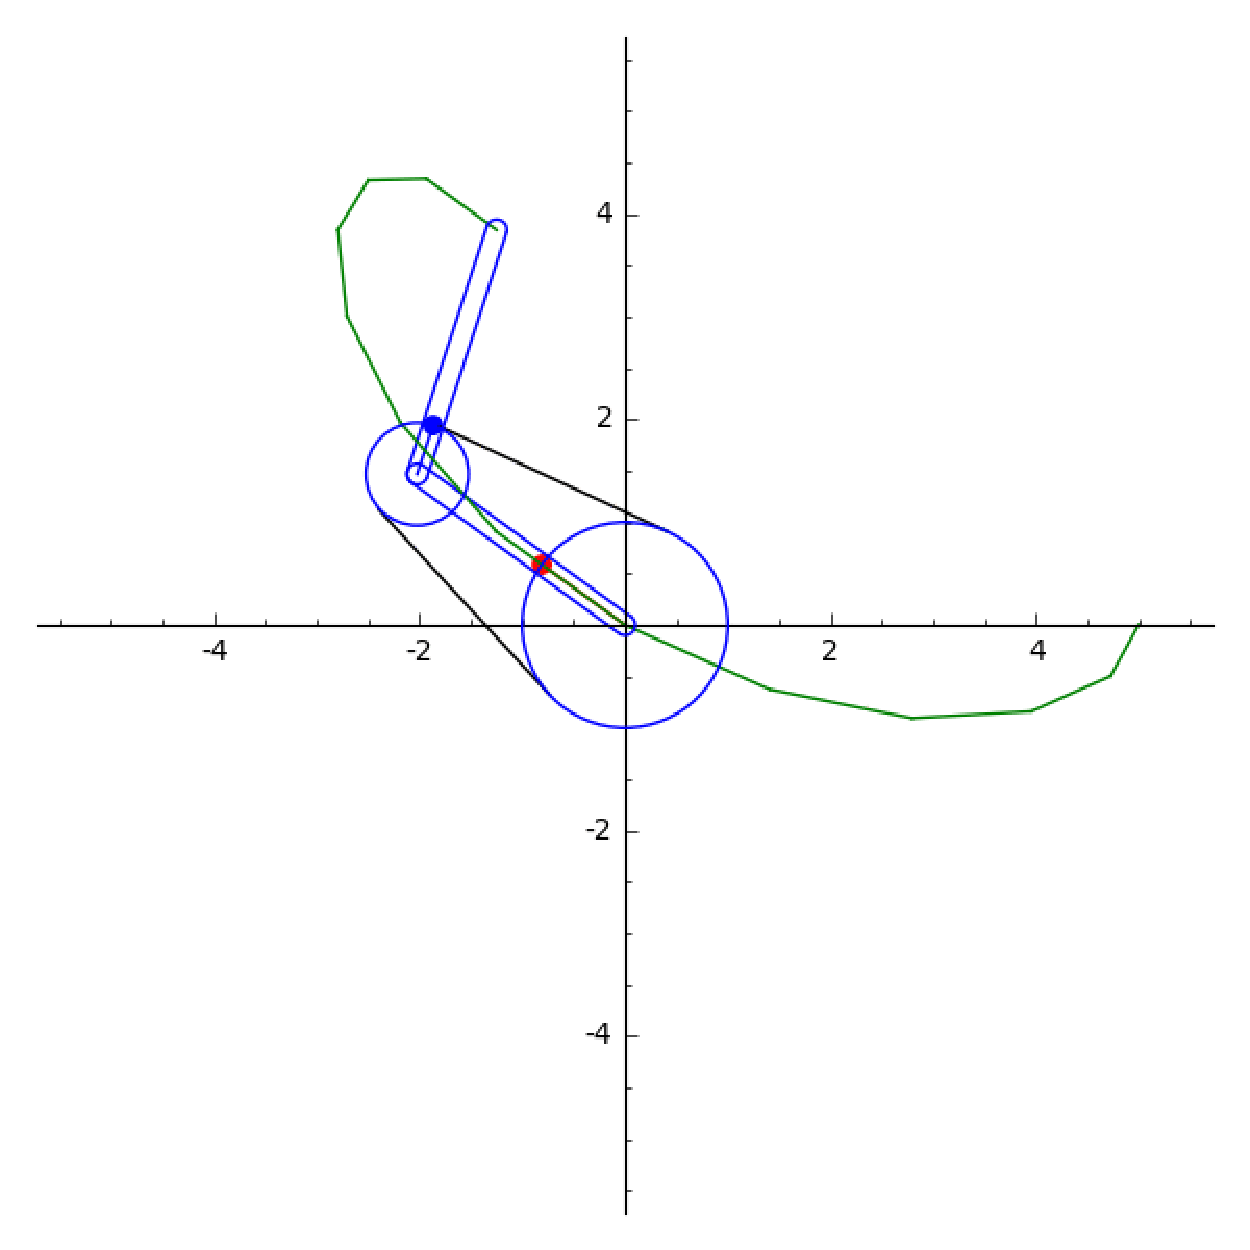
\includegraphics[scale=0.5]{tri13.eps}
\end{frame}

\begin{frame}
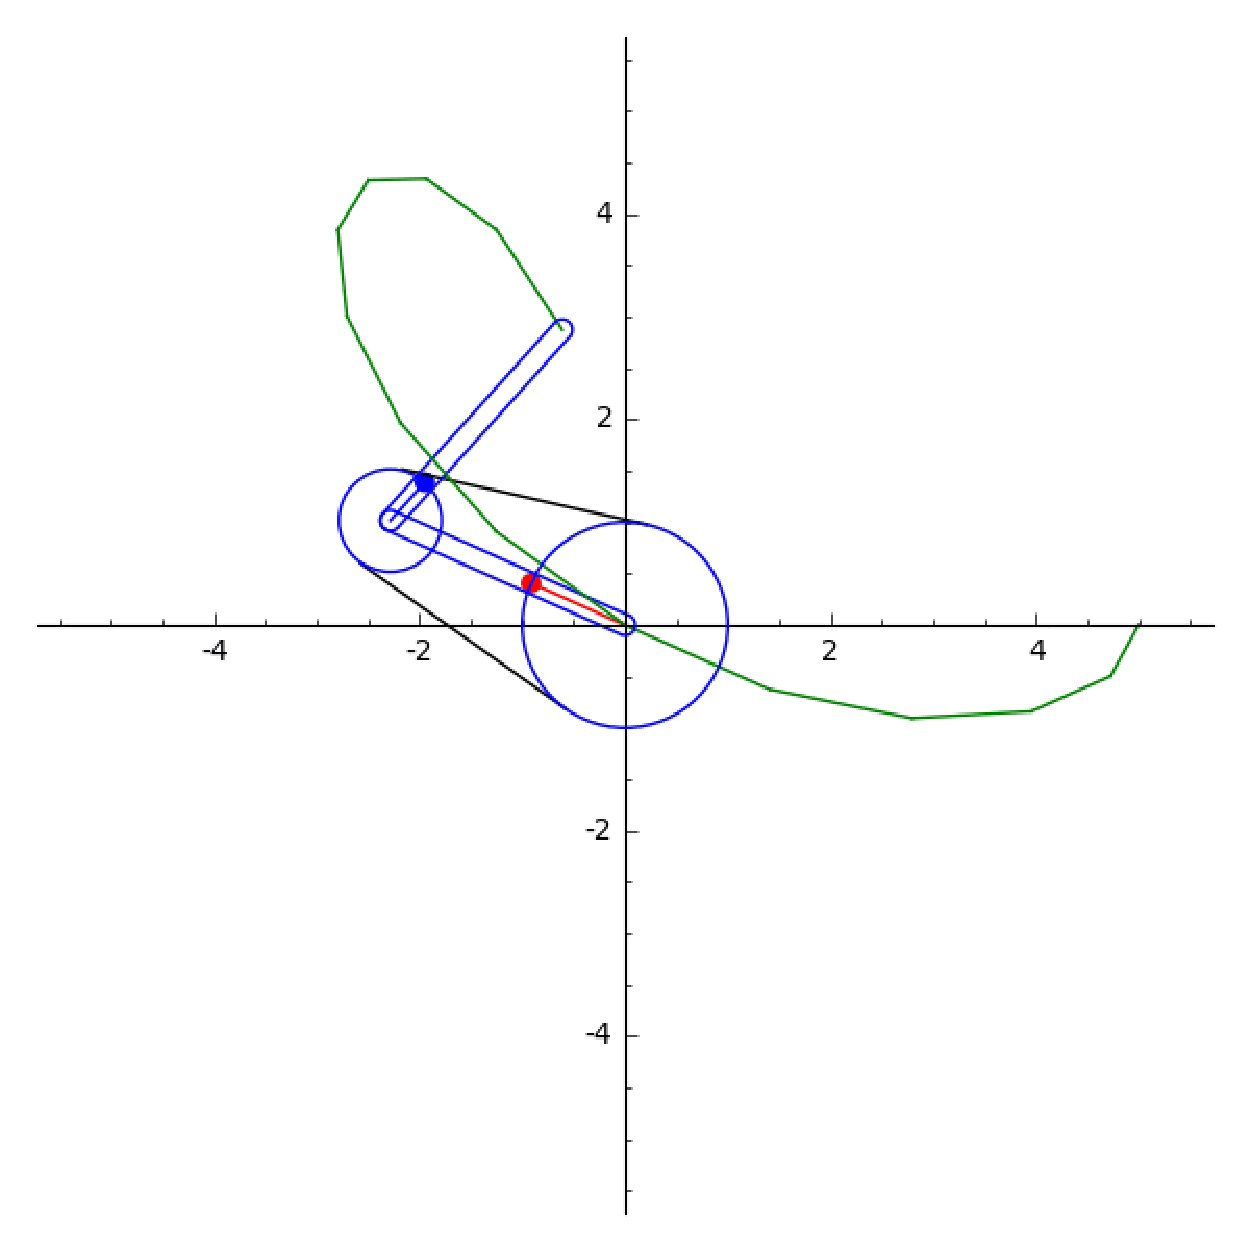
\includegraphics[scale=0.5]{tri14.eps}
\end{frame}

\begin{frame}
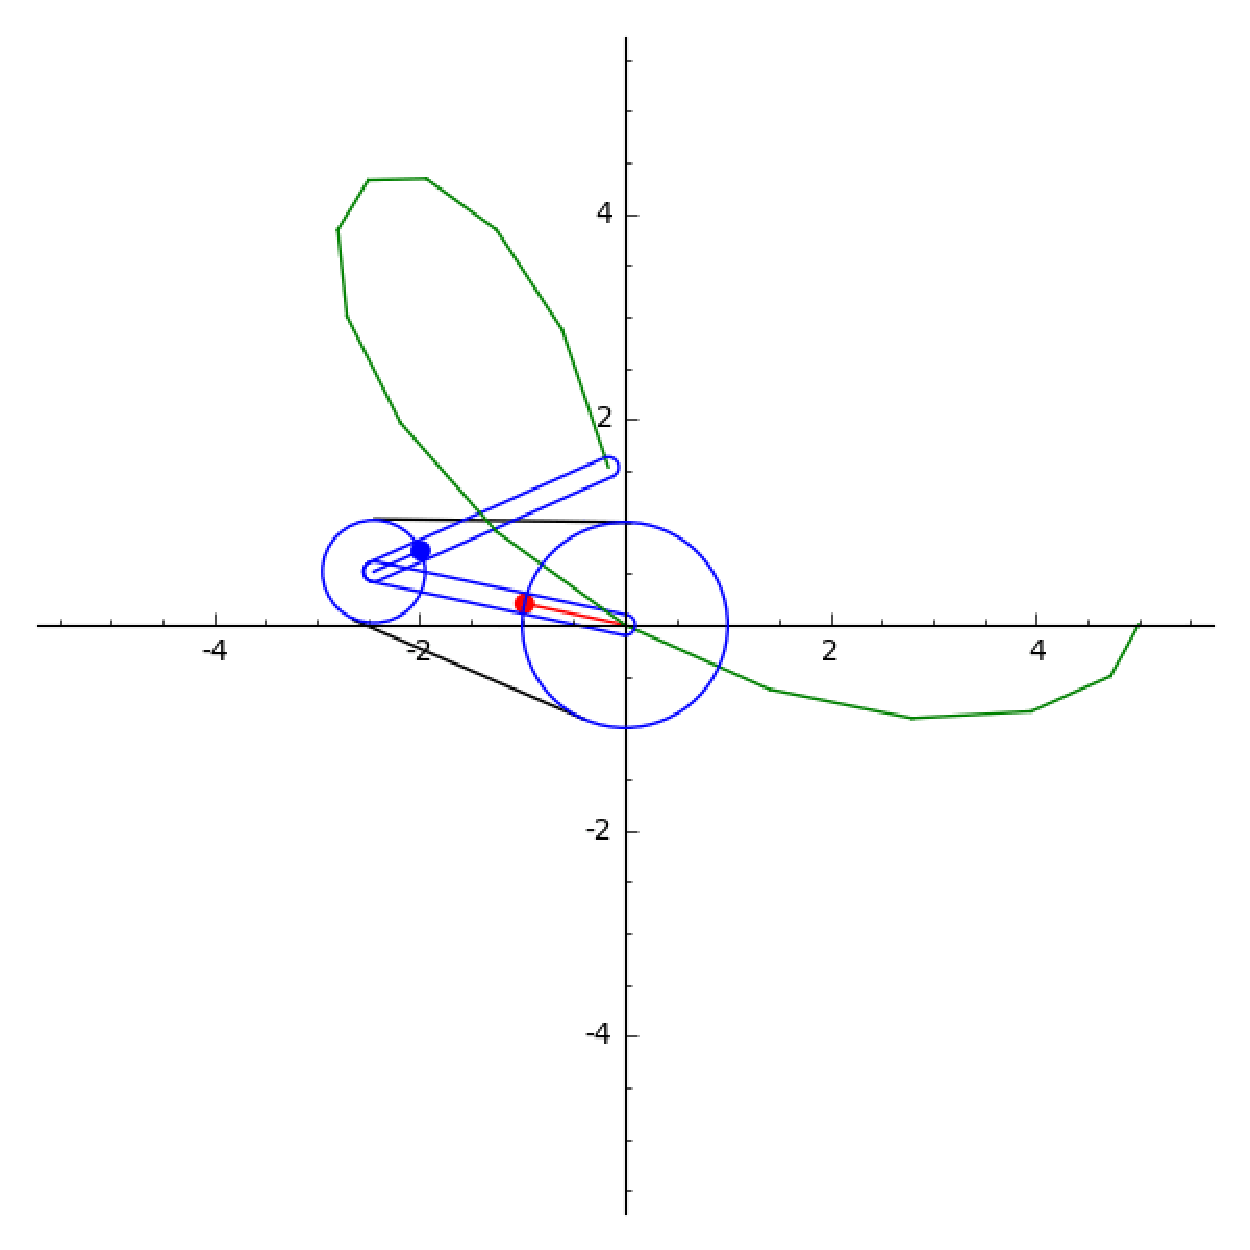
\includegraphics[scale=0.5]{tri15.eps}
\end{frame}

\begin{frame}
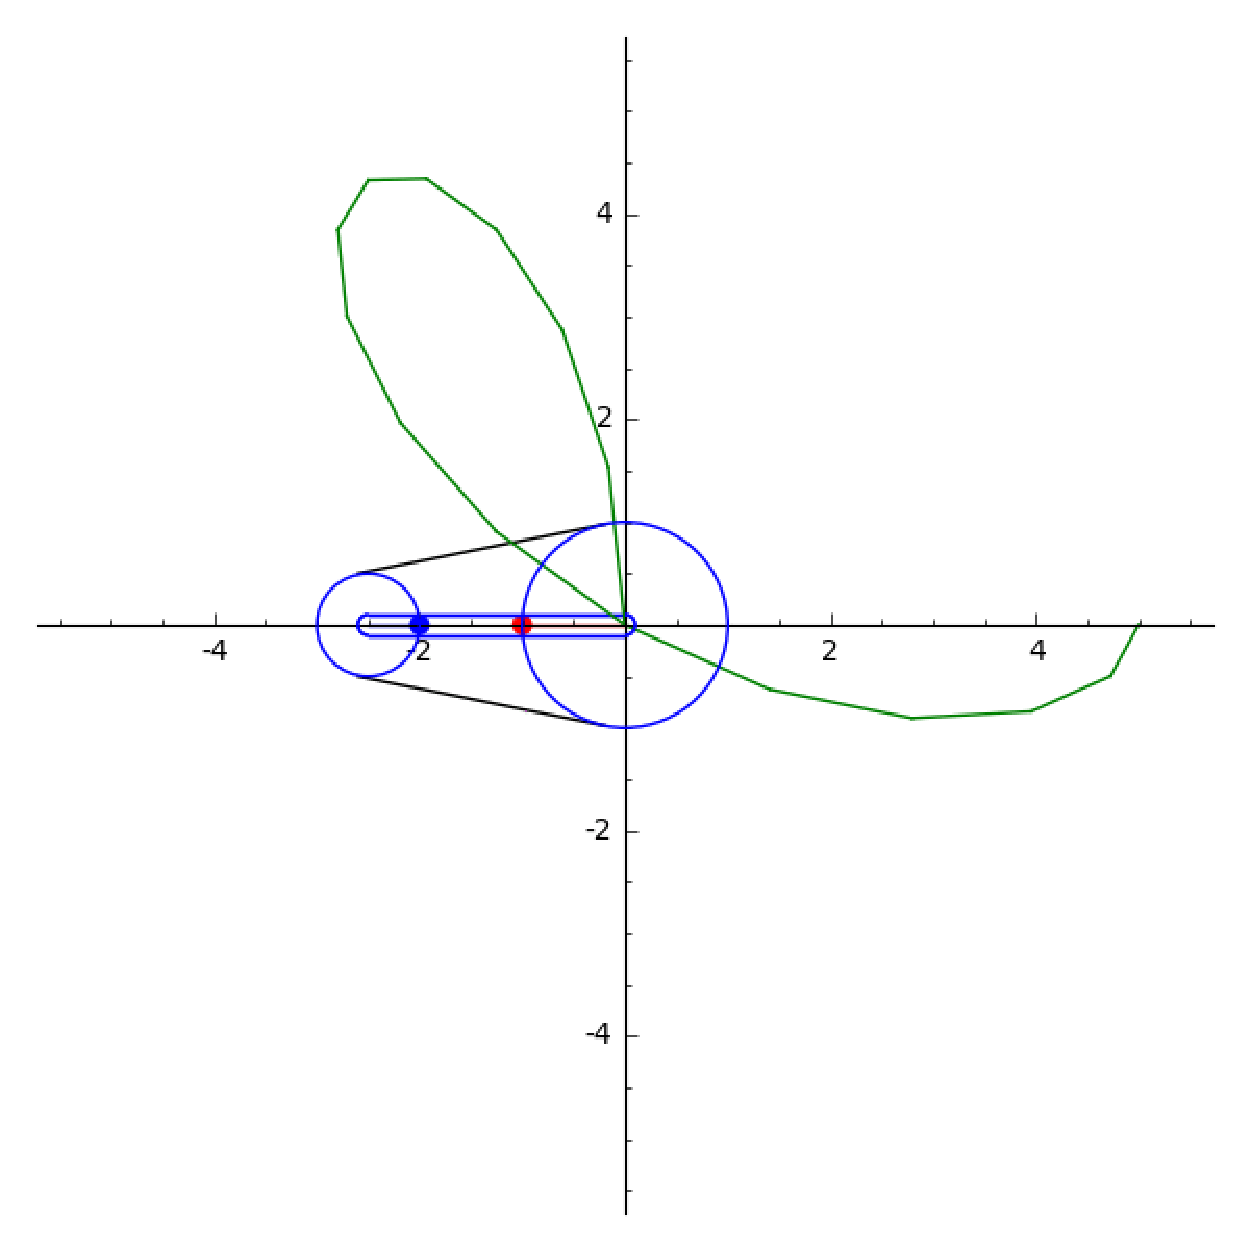
\includegraphics[scale=0.5]{tri16.eps}
\end{frame}

\begin{frame}
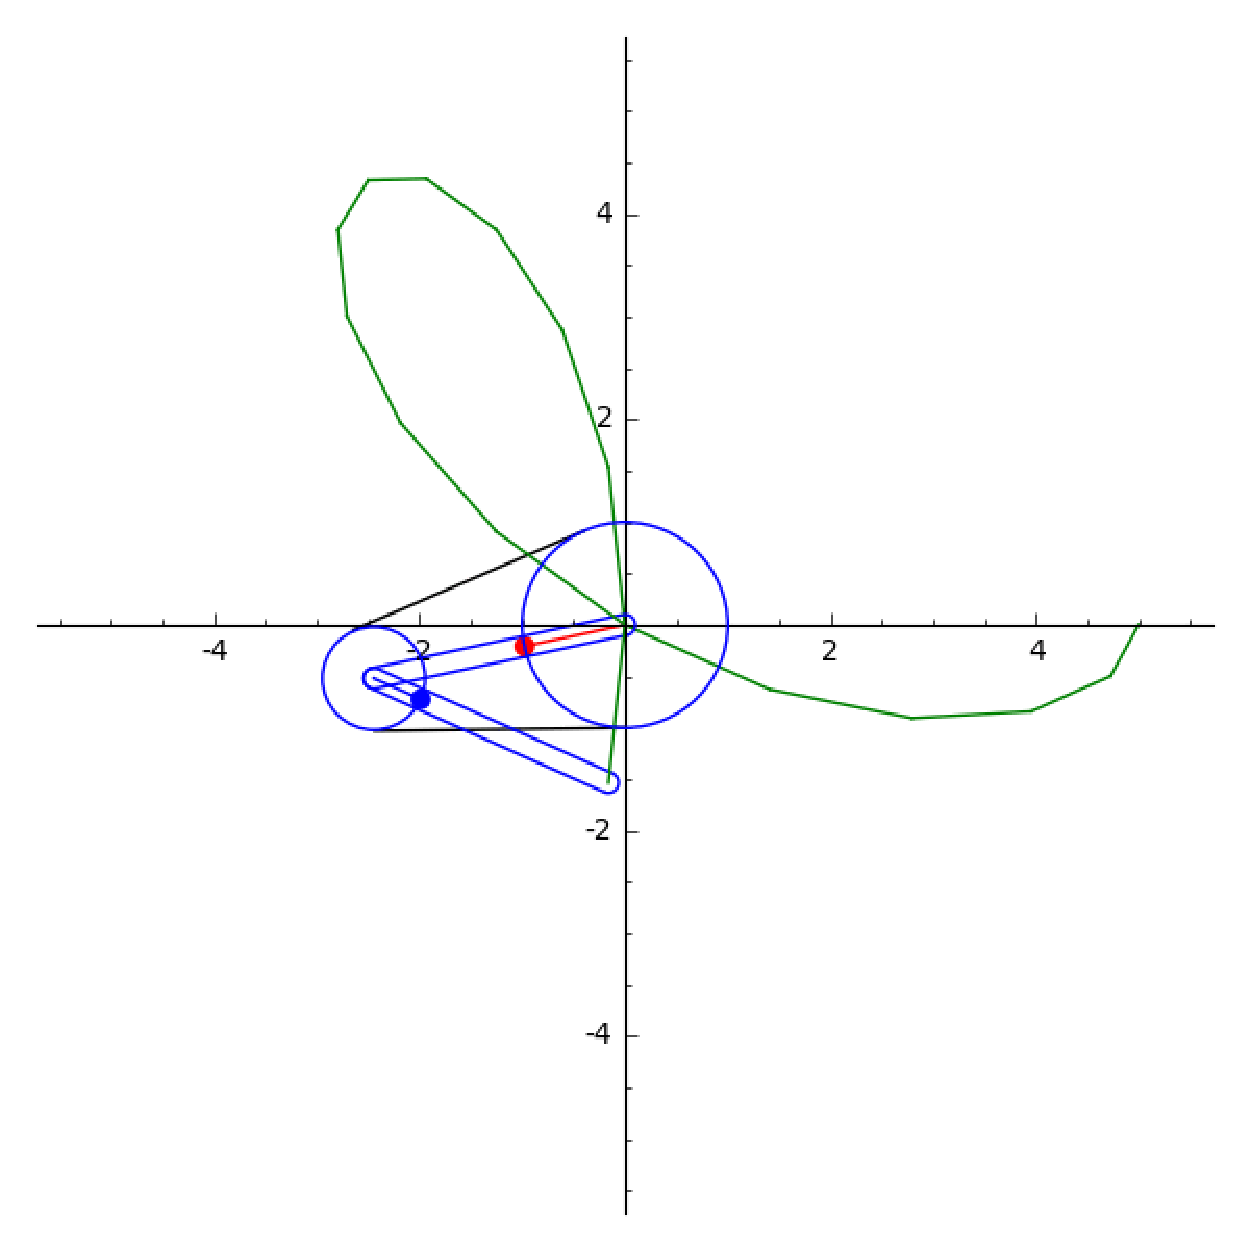
\includegraphics[scale=0.5]{tri17.eps}
\end{frame}

\begin{frame}
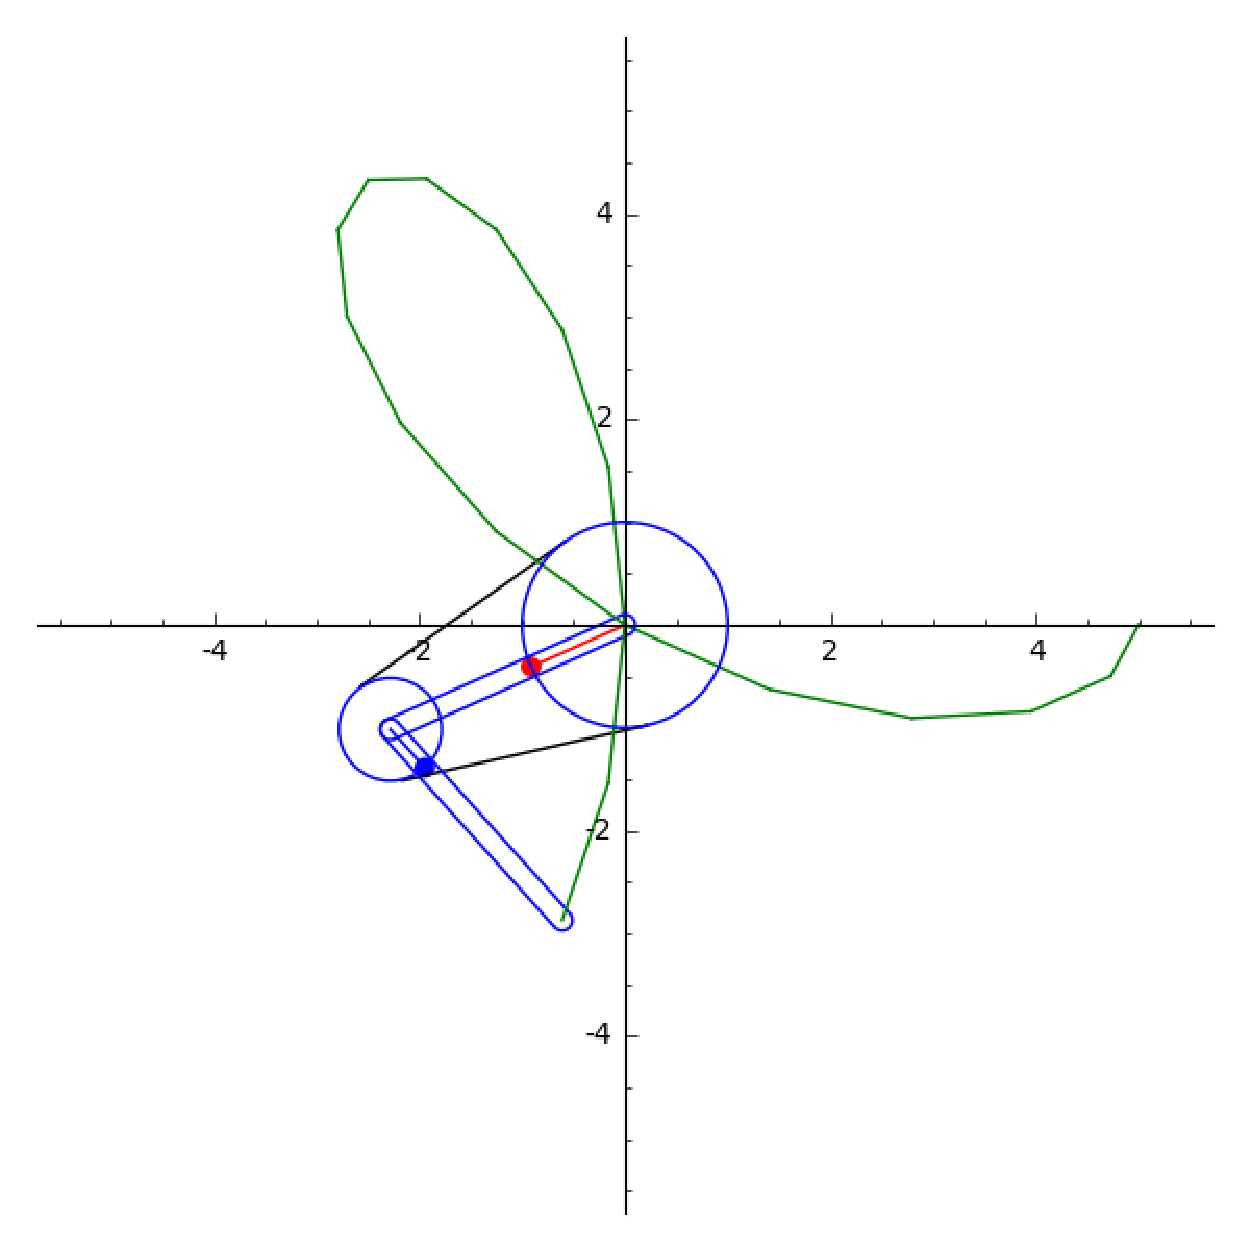
\includegraphics[scale=0.5]{tri18.eps}
\end{frame}

\begin{frame}
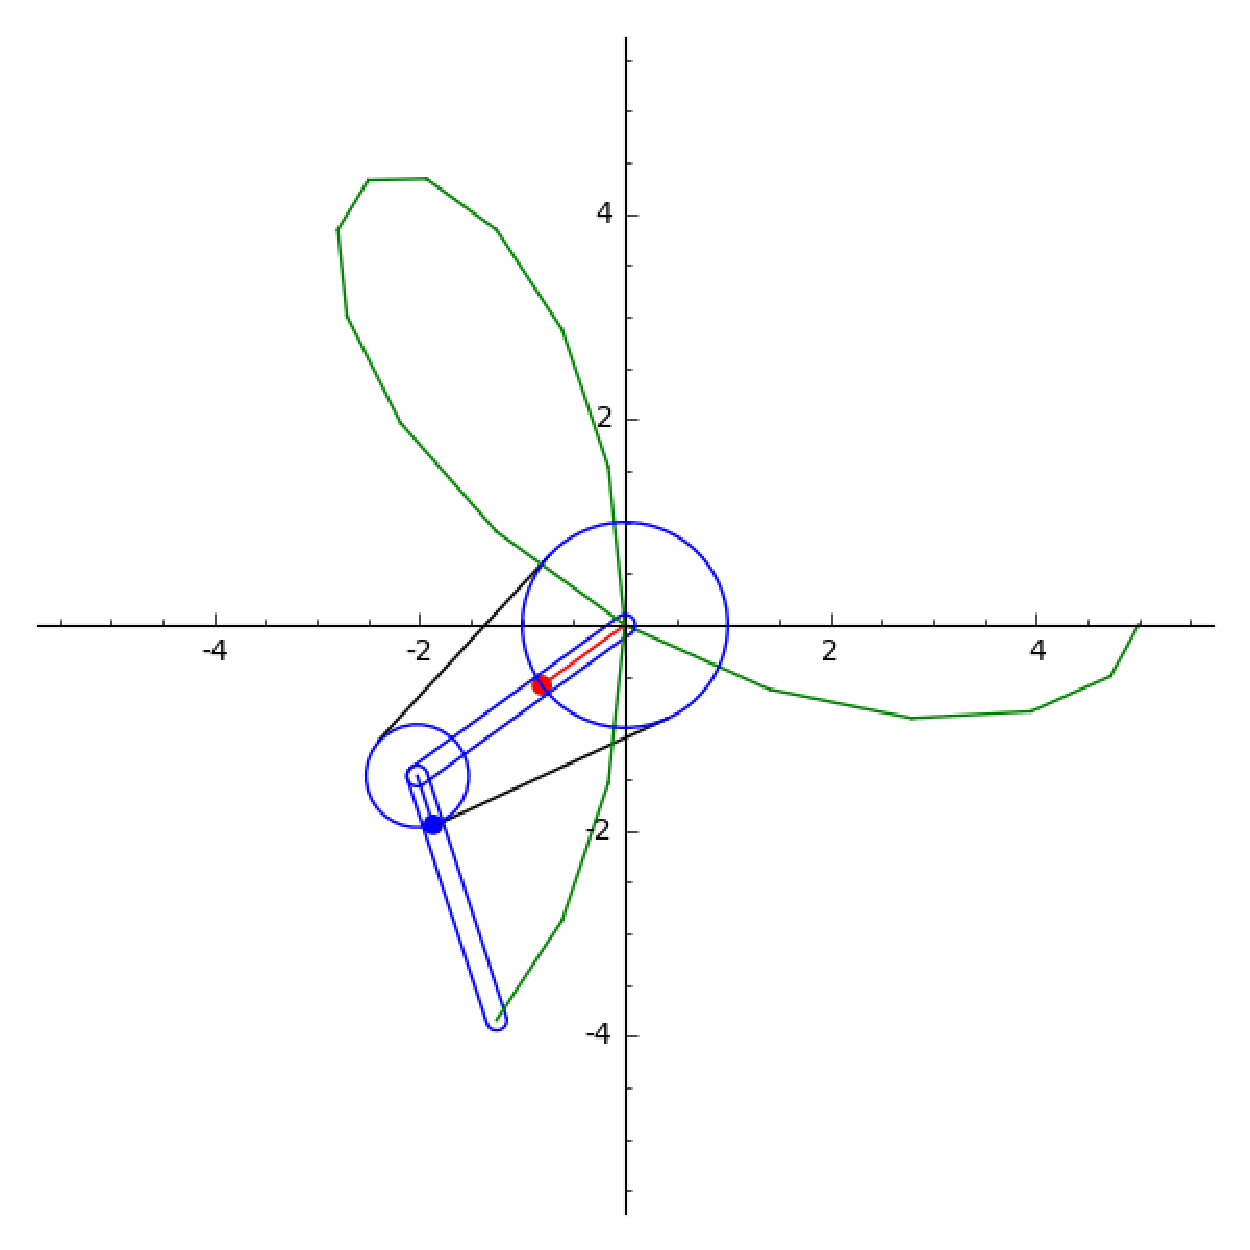
\includegraphics[scale=0.5]{tri19.eps}
\end{frame}

\begin{frame}
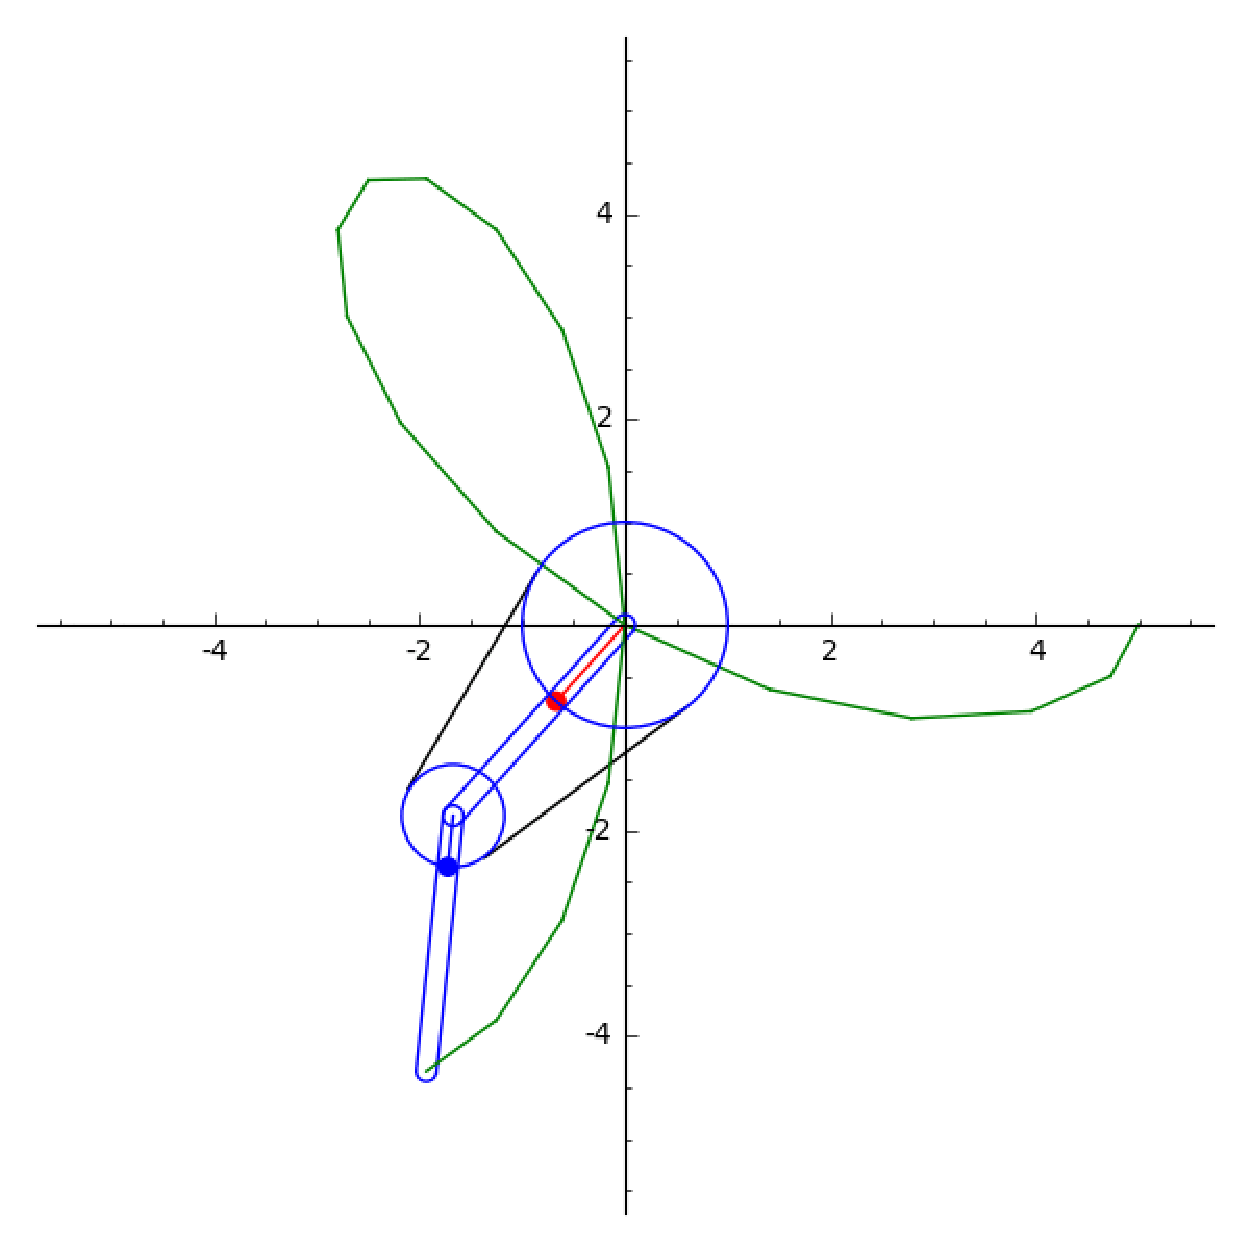
\includegraphics[scale=0.5]{tri20.eps}
\end{frame}

\begin{frame}
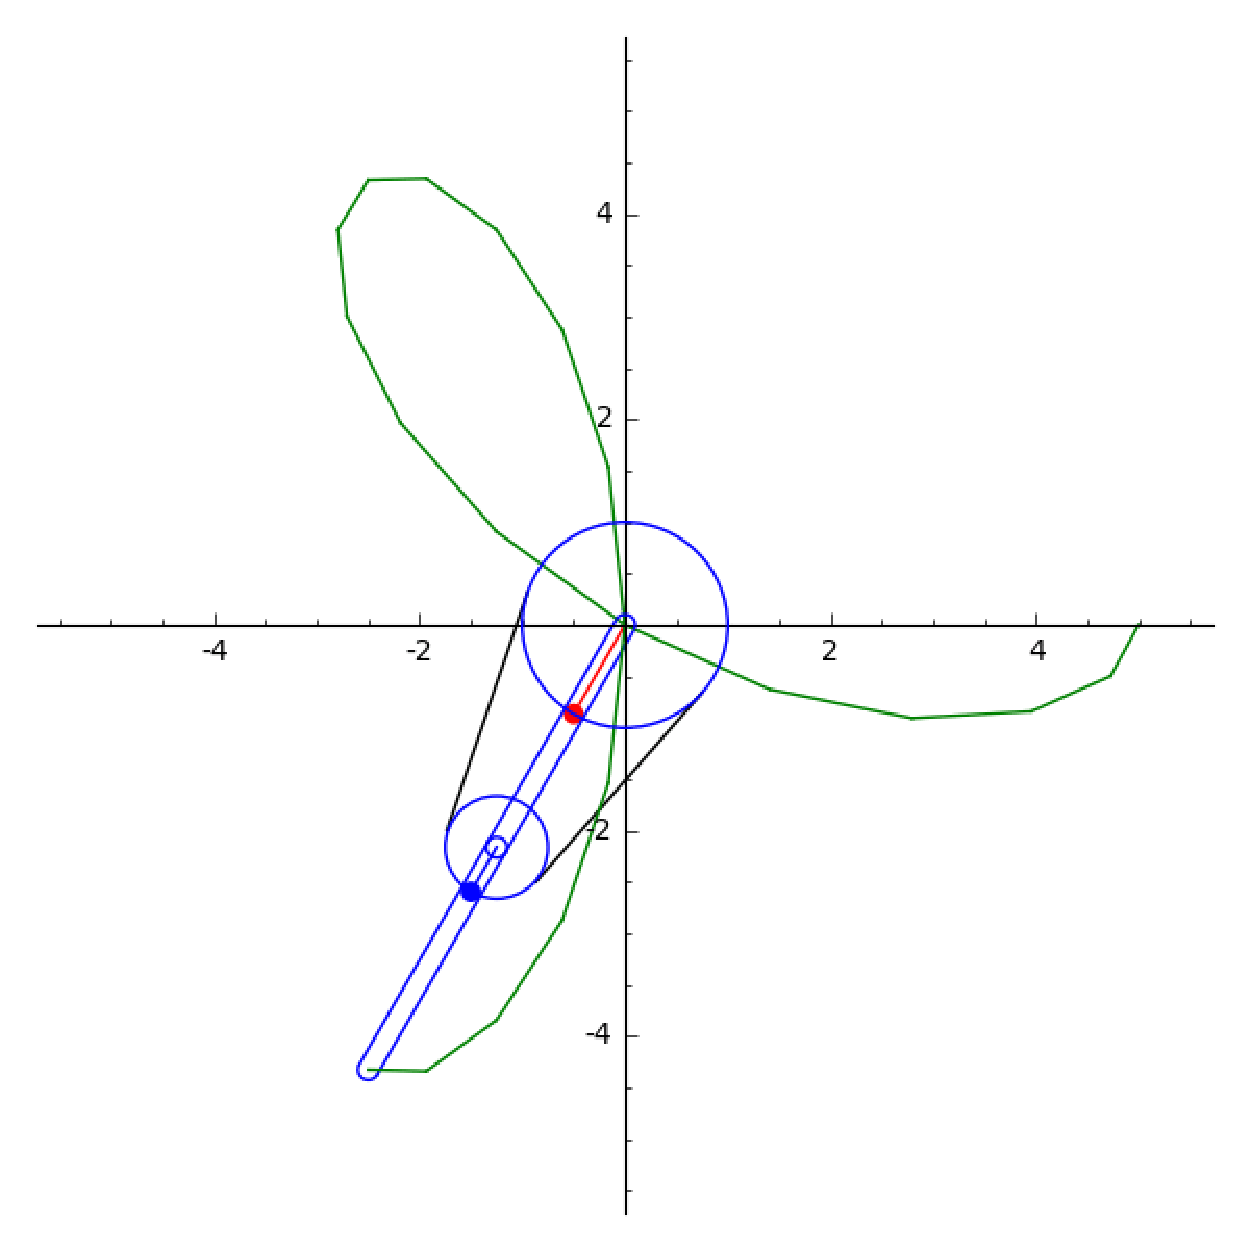
\includegraphics[scale=0.5]{tri21.eps}
\end{frame}

\begin{frame}
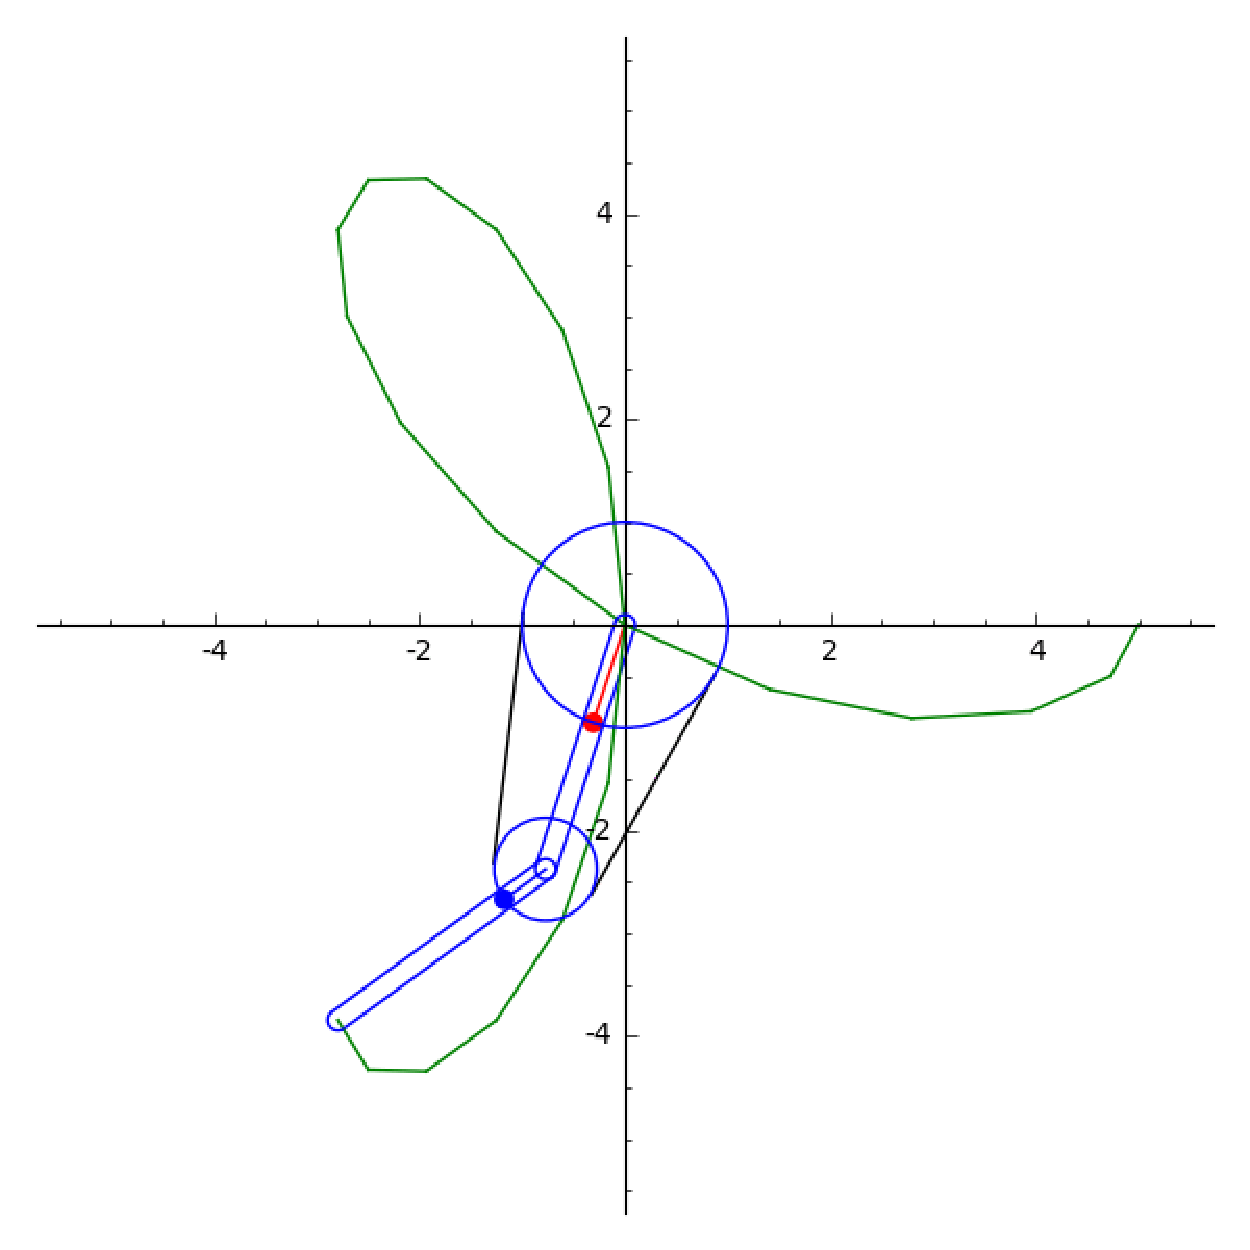
\includegraphics[scale=0.5]{tri22.eps}
\end{frame}

\begin{frame}
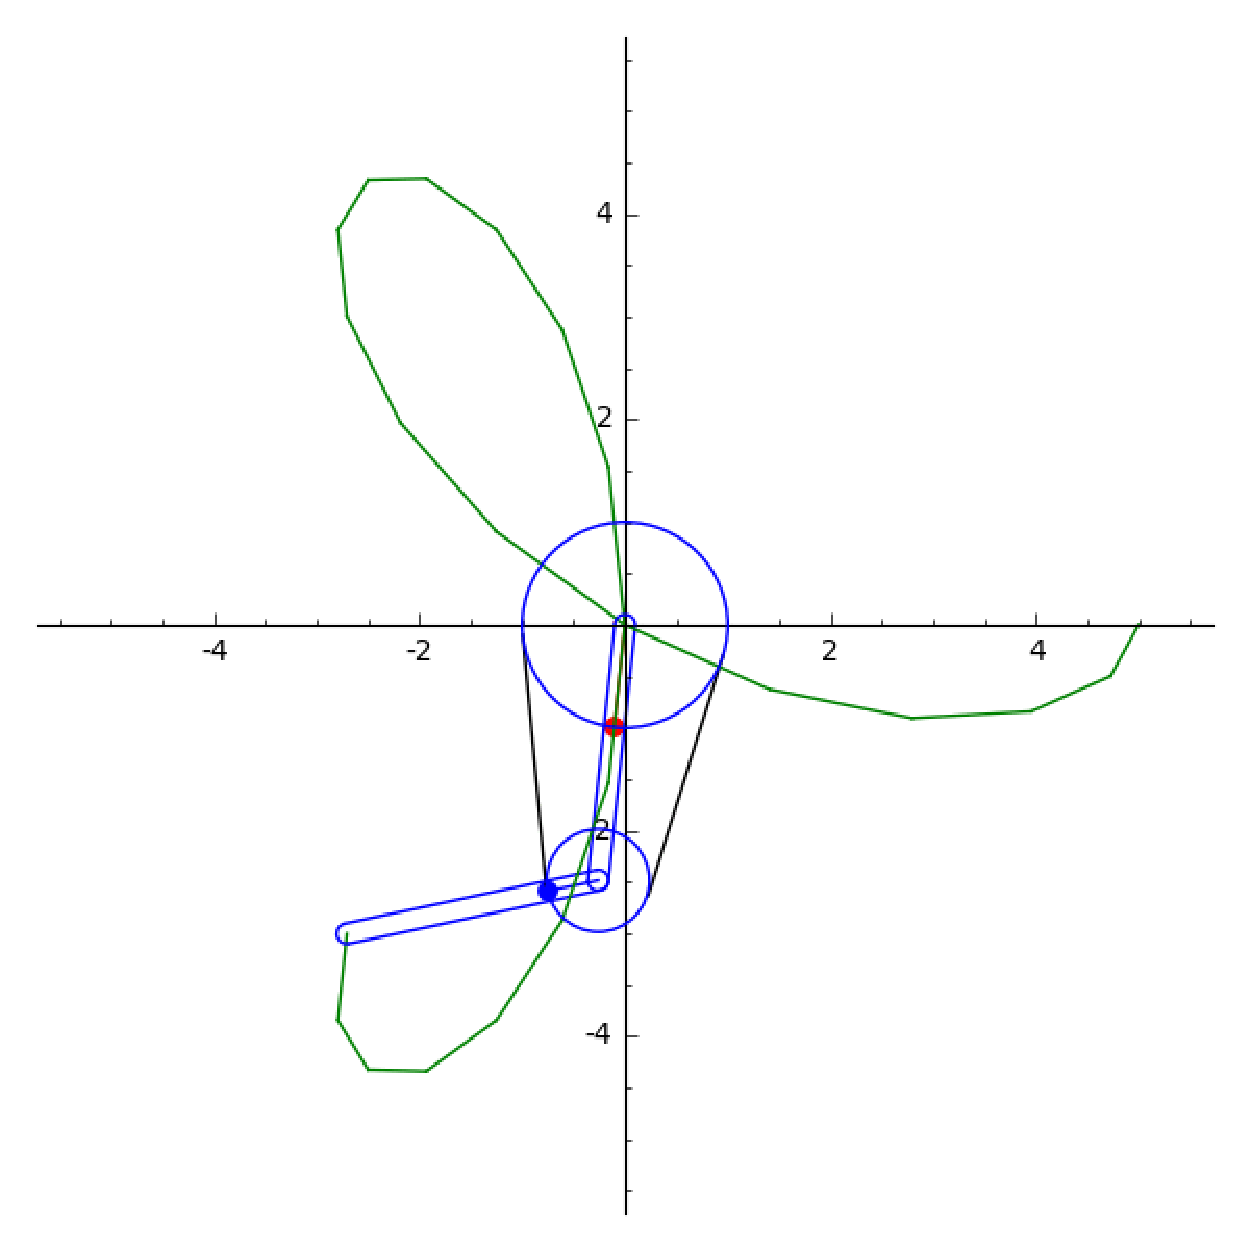
\includegraphics[scale=0.5]{tri23.eps}
\end{frame}

\begin{frame}
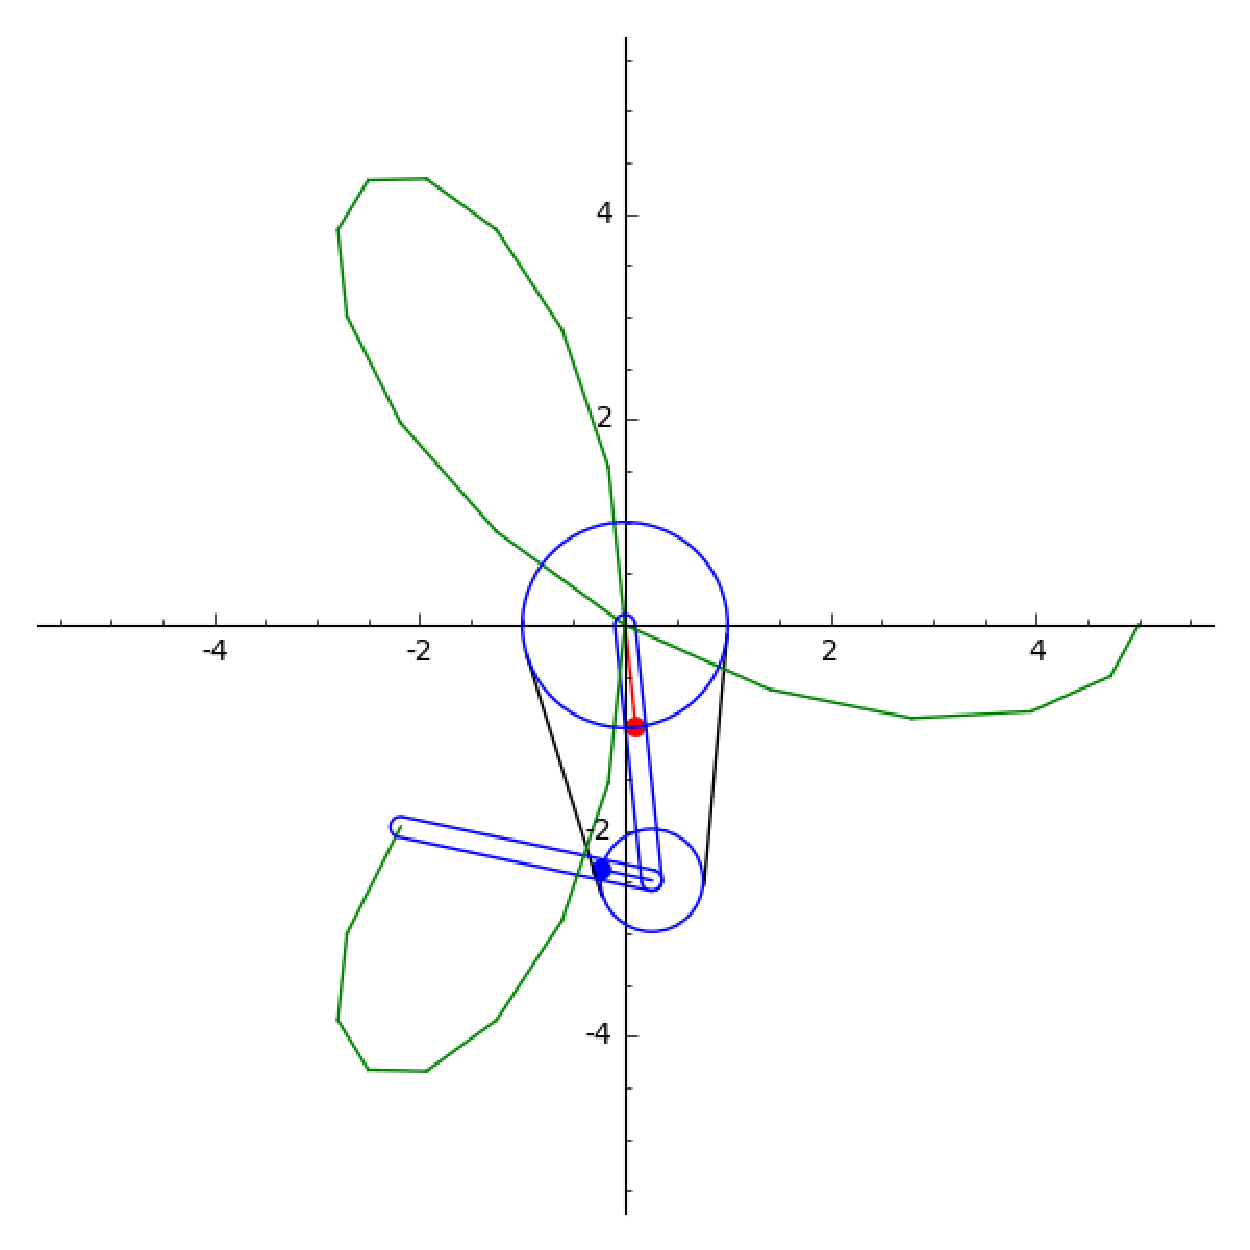
\includegraphics[scale=0.5]{tri24.eps}
\end{frame}

\begin{frame}
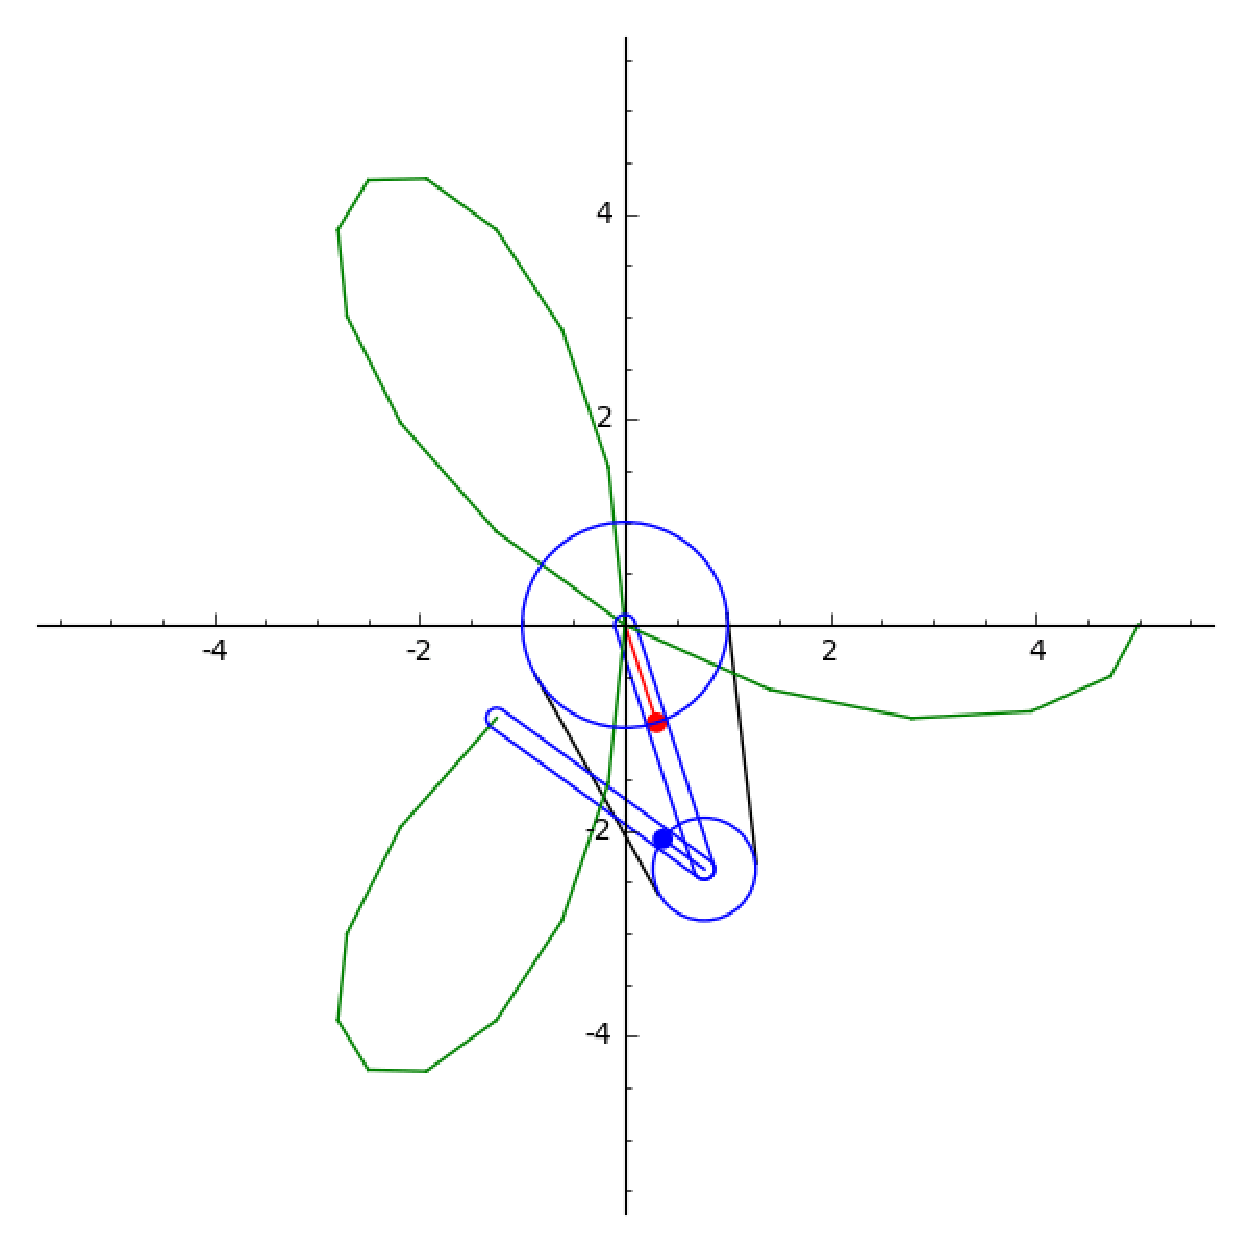
\includegraphics[scale=0.5]{tri25.eps}
\end{frame}
\begin{frame}
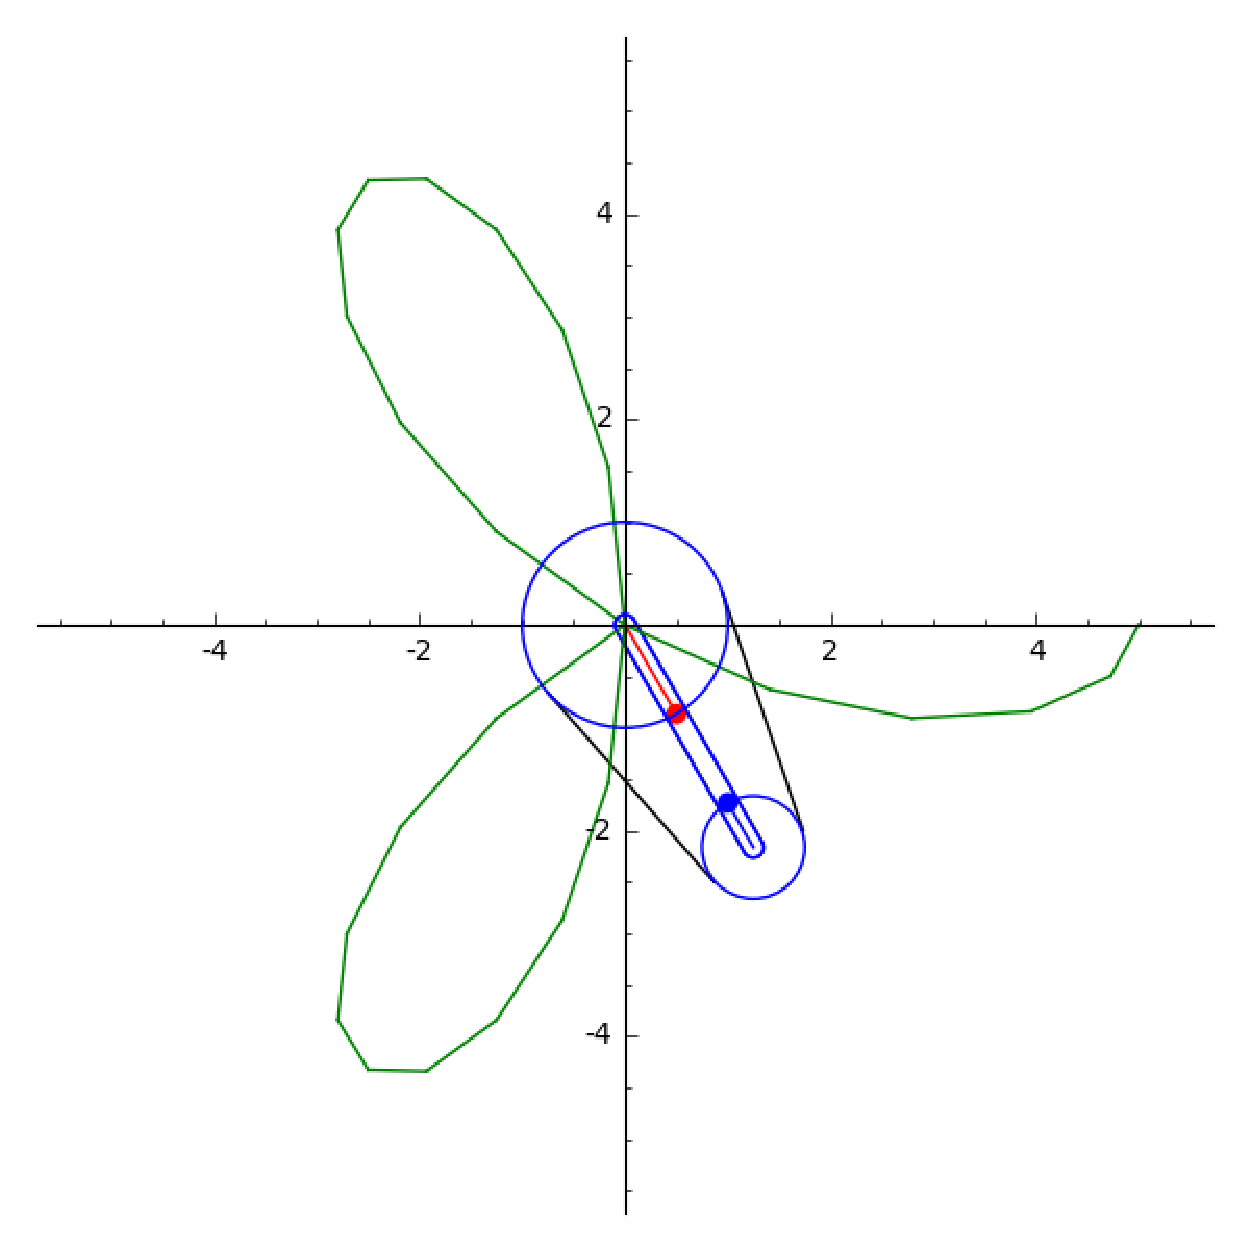
\includegraphics[scale=0.5]{tri26.eps}
\end{frame}

\begin{frame}
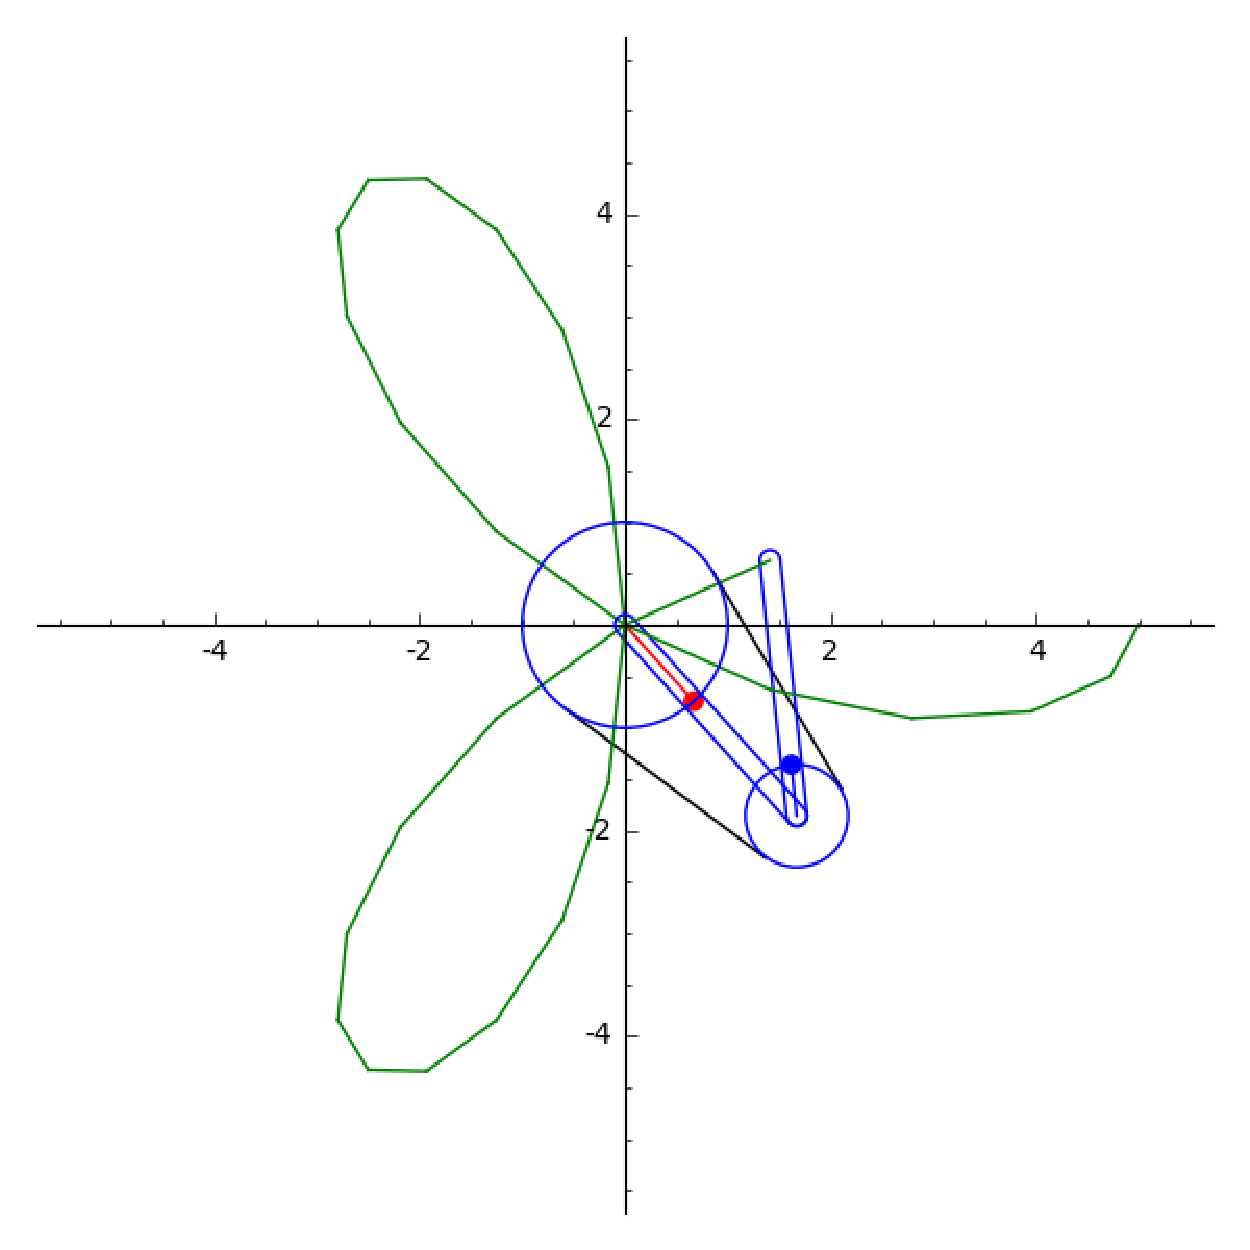
\includegraphics[scale=0.5]{tri27.eps}
\end{frame}

\begin{frame}
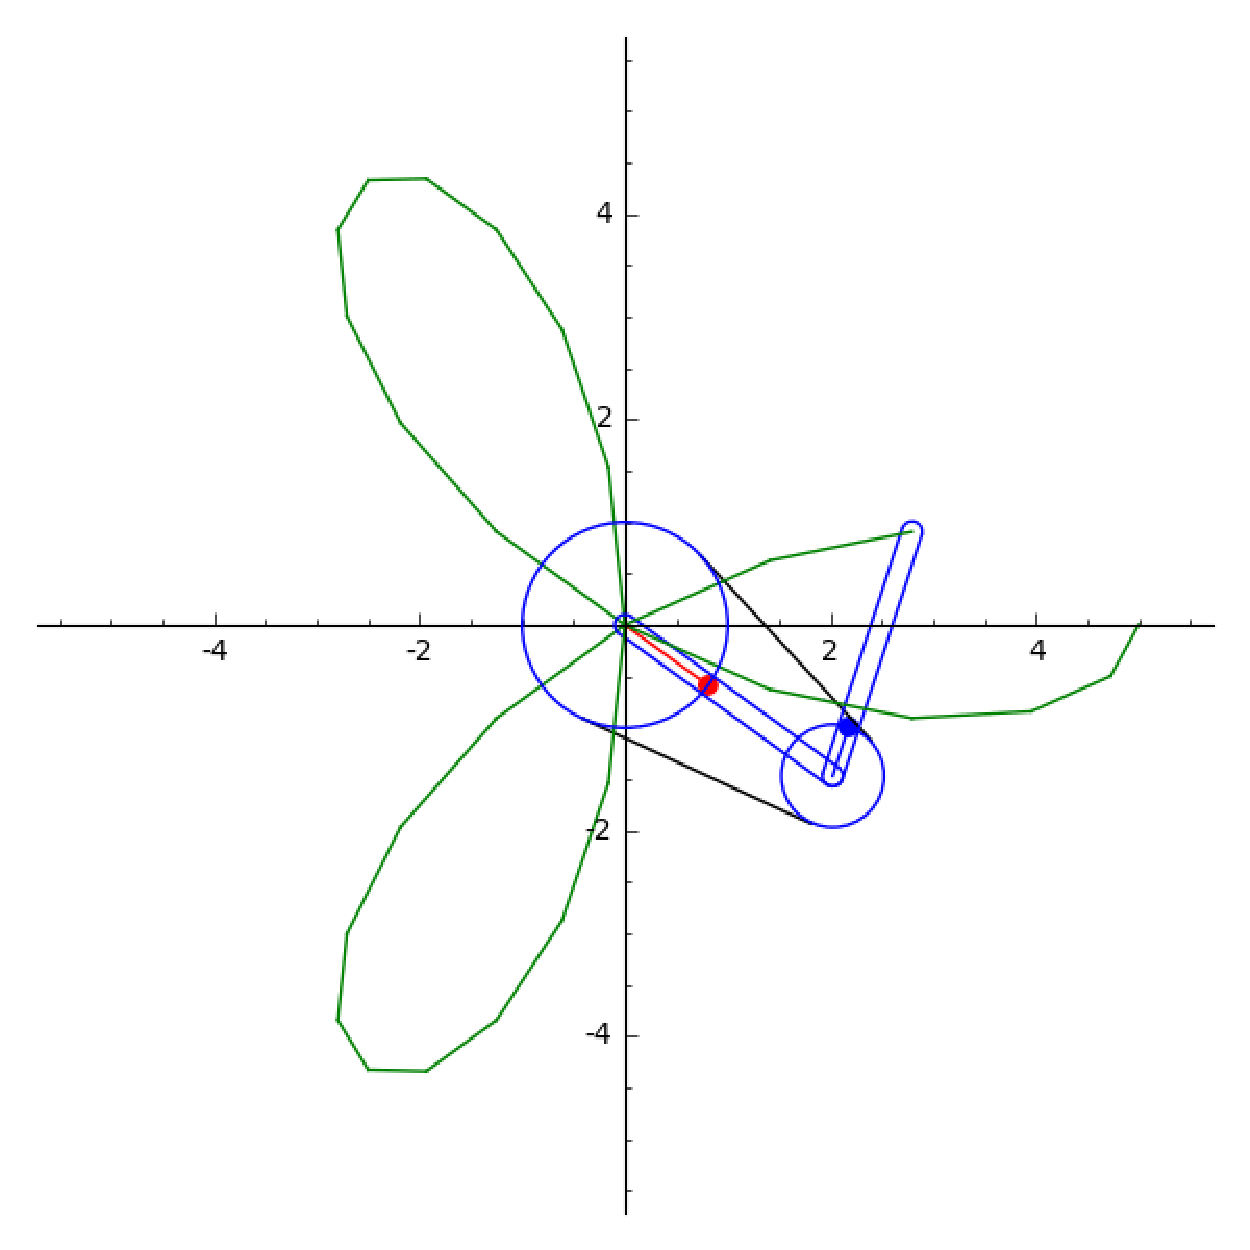
\includegraphics[scale=0.5]{tri28.eps}
\end{frame}

\begin{frame}
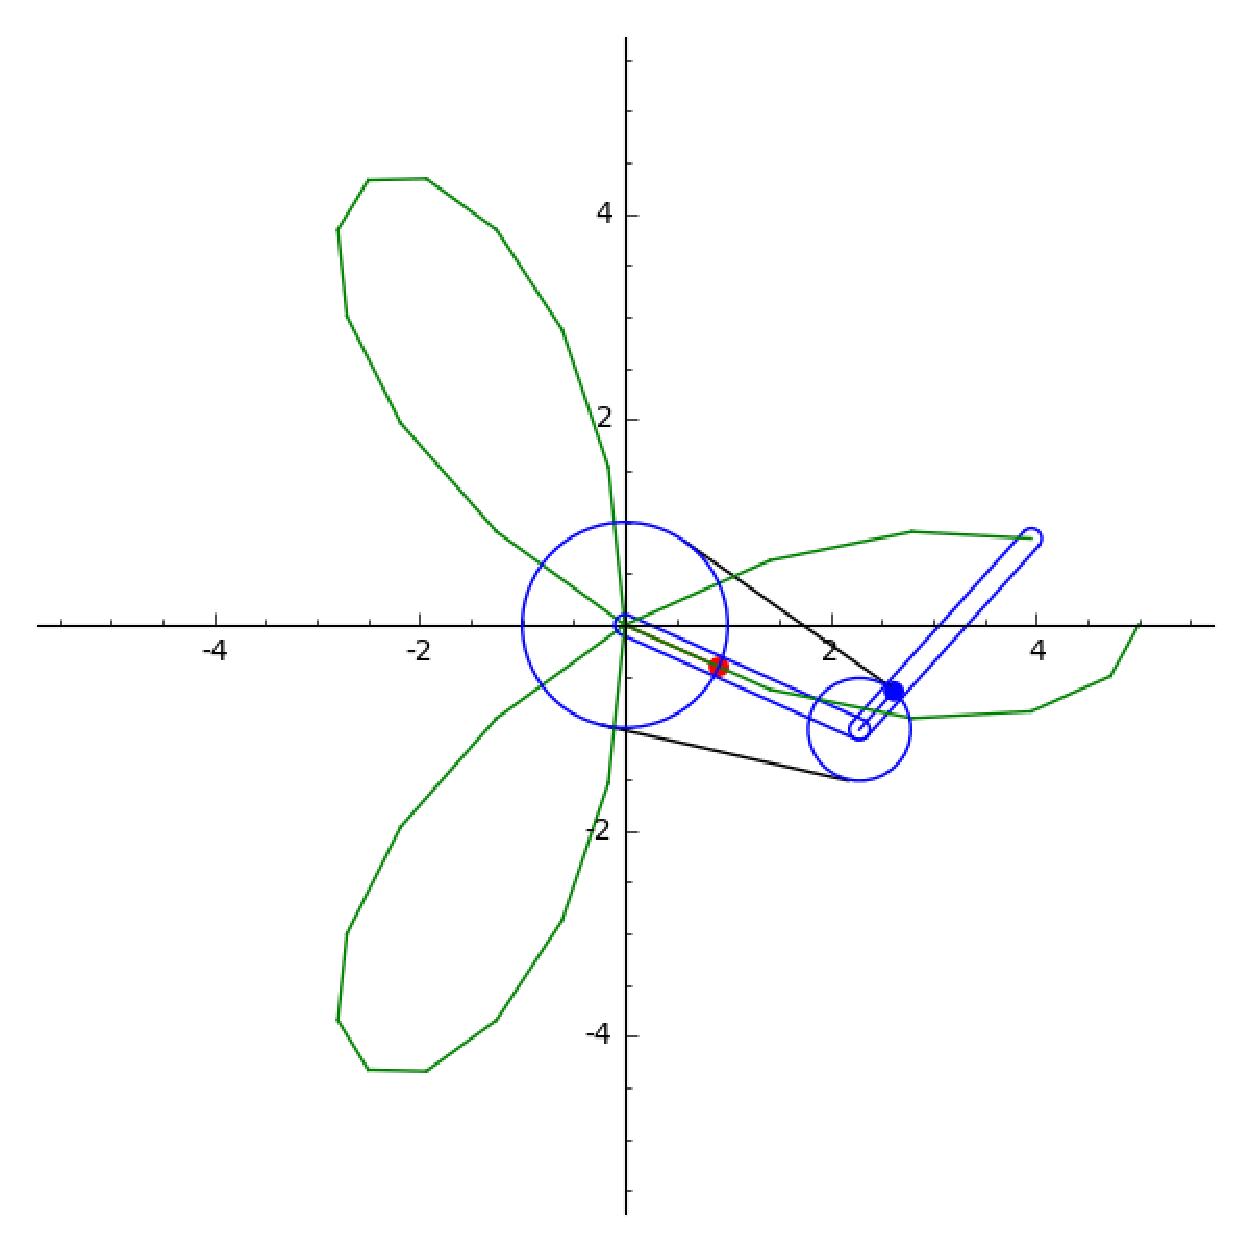
\includegraphics[scale=0.5]{tri29.eps}
\end{frame}

\begin{frame}
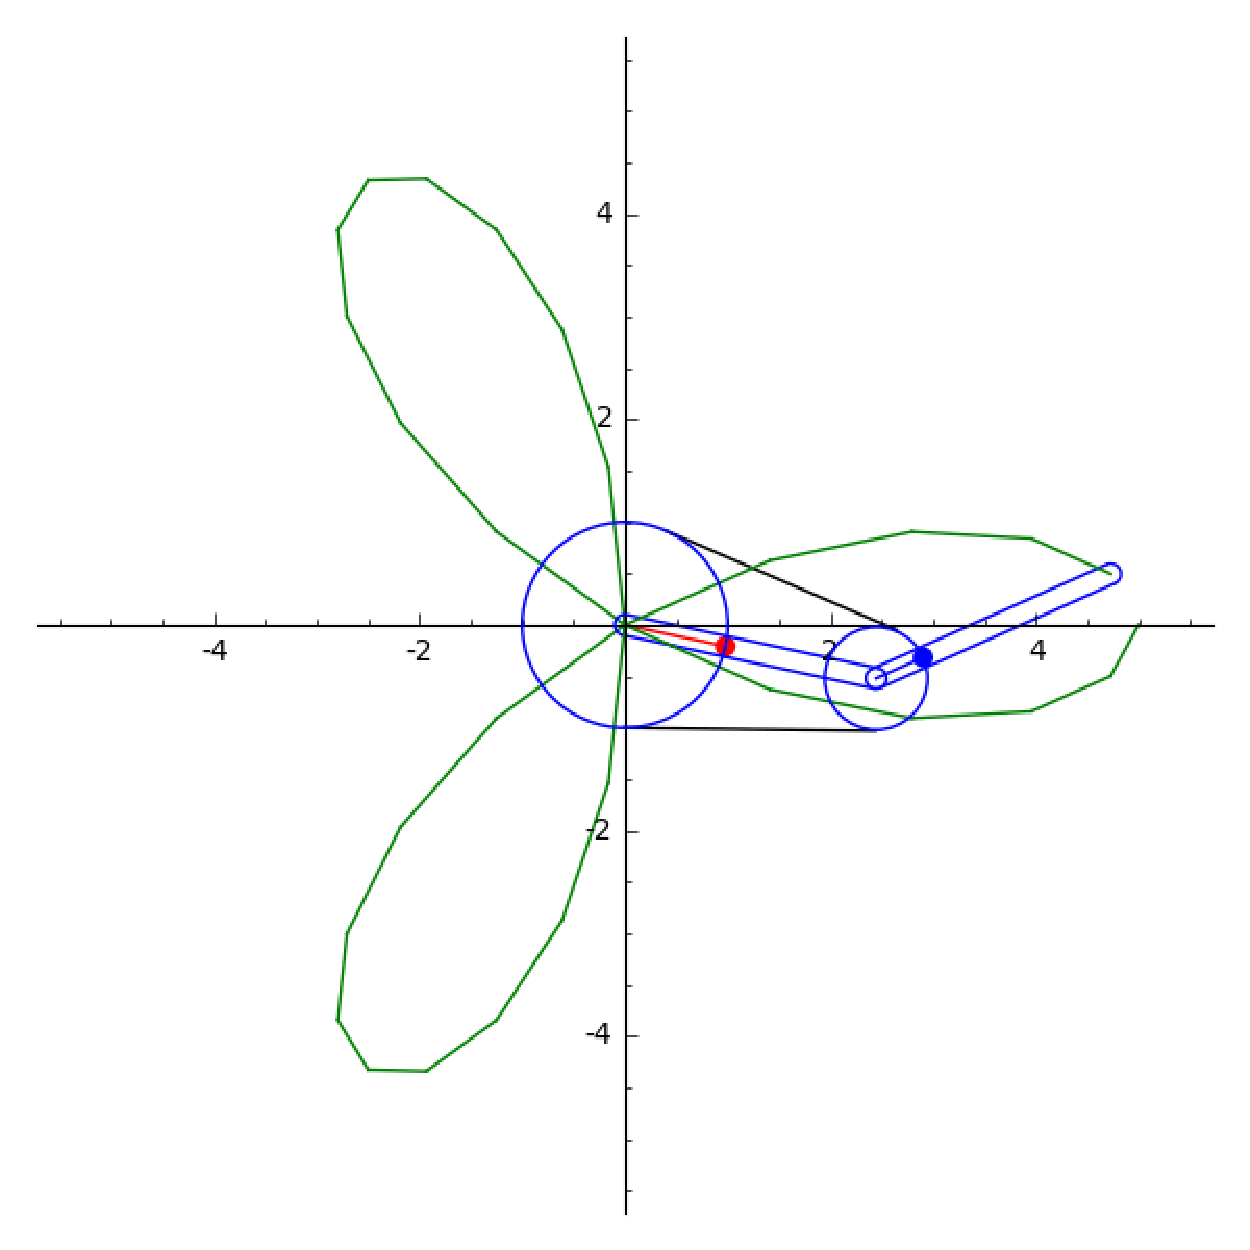
\includegraphics[scale=0.5]{tri30.eps}
\end{frame}

\begin{frame}
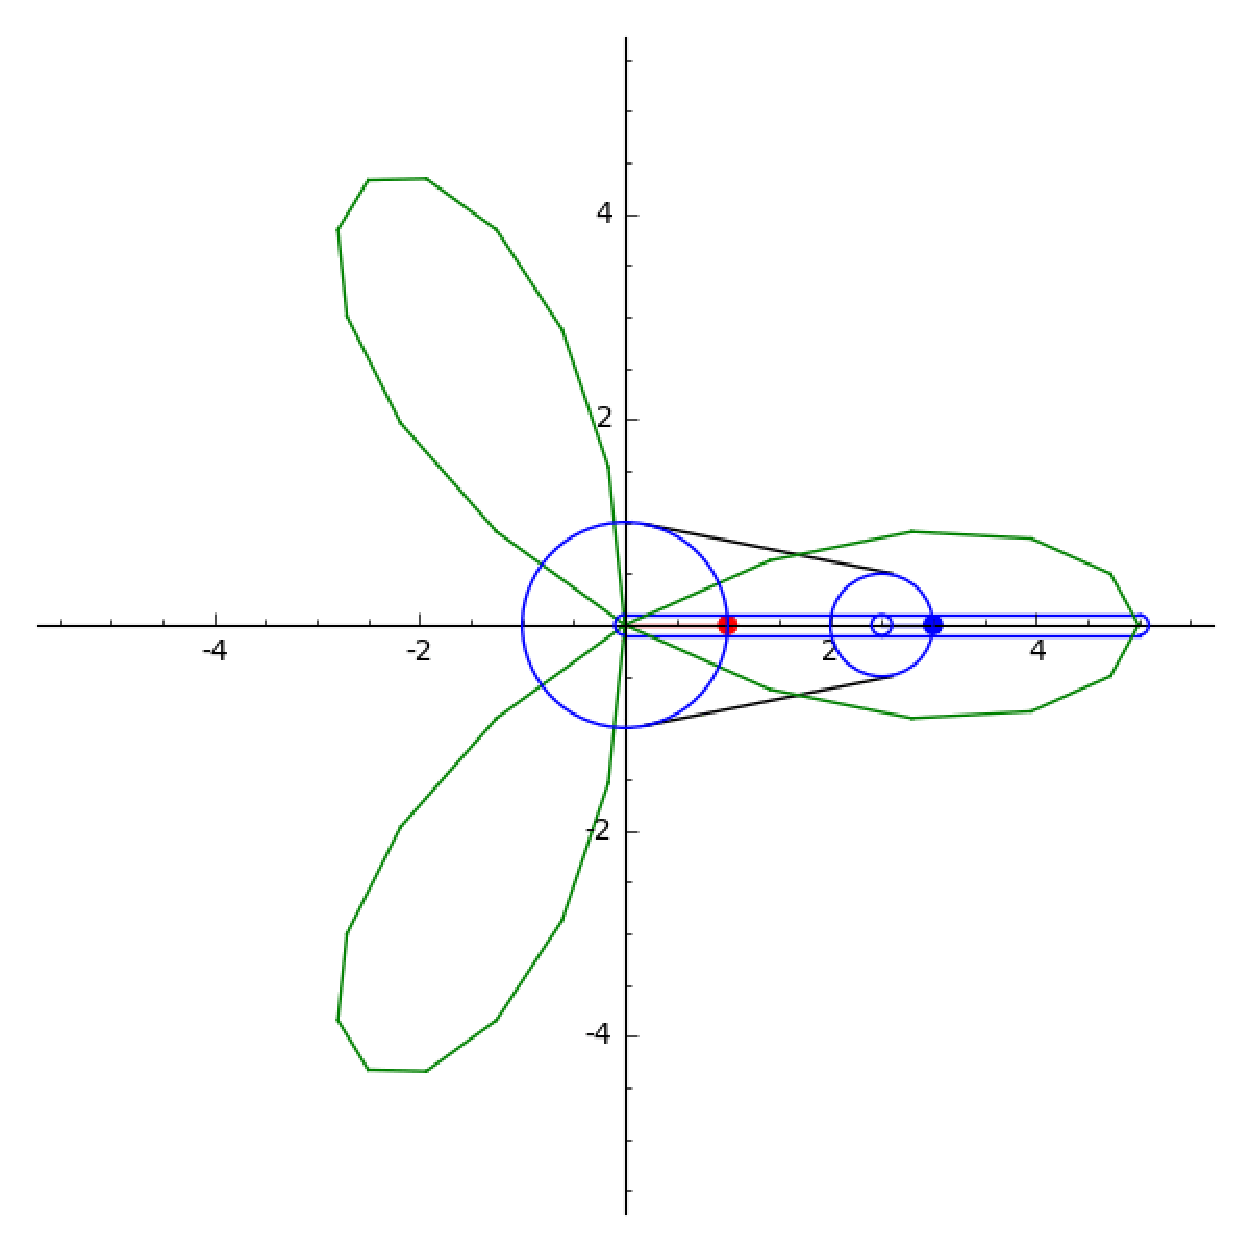
\includegraphics[scale=0.5]{tri31.eps}
\end{frame}

%======================================================================
\iffalse

\begin{frame}
\frametitle{Slide title}

\begin{itemize}
\item An unordered list
\item of things
\end{itemize}

\pause

\begin{enumerate}
\item An ordered list
\item of things
\item not inside an example environment...
\pause
\item with a dramatic pause before \#4 is shown
\end{enumerate}

\end{frame}

%======================================================================

\begin{frame}
\frametitle{Proofs}

\begin{thm}
An even perfect square is a multiple of $4$.
\end{thm}

\begin{proof}
Left to the reader.
\end{proof}

\begin{cor}
An integer of the form $4k+2$ is not a perfect square.
\end{cor}

\end{frame}

%======================================================================
%                        GRAPHICS EXAMPLES
%======================================================================

% Whole-frame graphics
\begin{frame}[plain]
\begin{center}

\includegraphics[keepaspectratio=true,height=0.95\paperheight]{fig1}
%
\includegraphics[keepaspectratio=true,width=0.95\paperwidth]{fig1}
\end{center}
\end{frame}

% Note: "fig1" in the command above is the filename.  Latex will
% search for various extensions, including:
%   PDF (best option for vector graphics)
%   PNG (best option for pixel-perfect images, e.g. screenshots or images of text)
%   JPG (best option for photographs)



% Multiple centered, captioned figures, top to bottom
\begin{frame}
\begin{center}
\begin{figure}

\includegraphics[keepaspectratio=true,height=0.3\paperheight]{fig1}
\caption{After MCL}
\end{figure}
\begin{figure}

\includegraphics[keepaspectratio=true,height=0.3\paperheight]{fig2}
\caption{Before MCL}
\end{figure}
\end{center}
\end{frame}

% Multiple captioned figures, side by side
\begin{frame}
\begin{columns}

\begin{column}{0.5\textwidth}
    \begin{center}
        \begin{figure}
        
\includegraphics[keepaspectratio=true,width=0.4\paperwidth]{fig1}
        \caption{After MCL}
        \end{figure}
    \end{center}
\end{column}

\begin{column}{0.5\textwidth}
    \begin{center}
        \begin{figure}
        
\includegraphics[keepaspectratio=true,width=0.4\paperwidth]{fig2}
        \caption{Before MCL}
        \end{figure}
    \end{center}
\end{column}

\end{columns}
\end{frame}
\fi
%======================================================================
%                            LAST SLIDES
%======================================================================

% References

\setbeamertemplate{frametitle continuation}{\gdef\beamer@frametitle{}}
\frame[allowframebreaks]{
\frametitle{References}
\begin{thebibliography}{99}

\iffalse
\bibitem{taylor-wiles}
R. Taylor,  A. Wiles. \emph{Ring theoretic properties of certain Hecke algebras}. Ann. Math. \textbf{141} (1995), 553--572.
\fi

\bibitem{liu}
Liu Y, Michael McCarthy JJ.\emph{ Design of Mechanisms to Draw Trigonometric Plane Curves.} ASME. J. Mechanisms Robotics. 2017;9(2):024503-024503-8. doi:10.1115/1.4035882.  

\bibitem{sage}
SageMath, the Sage Mathematics Software System (Version 7.5.1),
   The Sage Developers, 2017, http://www.sagemath.org.

\bibitem{kempe-wiki}
Wikipedia contributors.\emph{ "Kempe's universality theorem."} Wikipedia, The Free Encyclopedia. Wikipedia, The Free Encyclopedia, 6 Sep. 2017. Web. 25 Oct. 2017.

\end{thebibliography}
\end{frame}

% Resist the temptation to end with a "thanks slide"; instead, either
% end with a list of references/credits, or with a simple slide of
% contact info (and optionally the title again).

\iffalse
\begin{frame}
\begin{center}
\Large{
Anne K. Example\\[0.8em]
\texttt{akexamp9@uic.edu}
}
\end{center}
\end{frame}
\fi


\end{document}
